\documentclass[11pt]{article}
\usepackage[T1]{fontenc}
\usepackage[utf8]{inputenc}
\usepackage{lmodern}
\usepackage[margin=1.05in]{geometry}
\usepackage{amsmath,amssymb,amsthm,mathtools}
\usepackage{microtype}
\usepackage{graphicx,tikz}
\usetikzlibrary{arrows.meta,calc,patterns,positioning,decorations.pathreplacing}
\usepackage{enumerate,booktabs}
\usepackage{xcolor}
\definecolor{linkblue}{RGB}{30,63,103}
\usepackage[colorlinks=true,linkcolor=linkblue,citecolor=linkblue,urlcolor=linkblue]{hyperref}
\hypersetup{pdftitle={Quenched SLE Universality for Weakly Disordered FK-Ising Interfaces},pdfauthor={OpenAI}}
\usepackage{bookmark}
\numberwithin{equation}{section}
\newtheorem{theorem}{Theorem}[section]
\newtheorem{proposition}[theorem]{Proposition}
\newtheorem{lemma}[theorem]{Lemma}
\newtheorem{corollary}[theorem]{Corollary}
\theoremstyle{definition}
\newtheorem{definition}[theorem]{Definition}
\newtheorem{assumption}[theorem]{Assumption}
\theoremstyle{remark}
\newtheorem{remark}[theorem]{Remark}
\newcommand{\E}{\mathbb E}
\renewcommand{\P}{\mathbb P}
\newcommand{\R}{\mathbb R}
\newcommand{\C}{\mathbb C}
\newcommand{\Hh}{\mathbb H}
\newcommand{\D}{\mathbb D}
\newcommand{\Z}{\mathbb Z}
\newcommand{\N}{\mathbb N}
\newcommand{\eps}{\varepsilon}
\newcommand{\norm}[1]{\left\lVert#1\right\rVert}
\newcommand{\abs}[1]{\left\lvert#1\right\rvert}
\newcommand{\dist}{\operatorname{dist}}
\newcommand{\diam}{\operatorname{diam}}
\newcommand{\osc}{\operatorname{osc}}
\newcommand{\SLE}{\mathrm{SLE}}
\newcommand{\FK}{\mathrm{FK}}
\newcommand{\id}{\mathrm{id}}
\newcommand{\ind}{\mathbf 1}
\newcommand{\dd}{\,\mathrm d}
\newcommand{\mathscr}{\mathcal}
\setlength{\emergencystretch}{2em}
\title{Quenched SLE Universality for Weakly Disordered FK--Ising Interfaces}
\author{OpenAI}
\date{October 5, 2026}
\begin{document}
\maketitle
\begin{abstract}
We prove that critical FK--Ising interfaces with sufficiently weak, symmetric,
independent two-valued bond disorder converge to chordal $\SLE_{16/3}$.
The disorder strength is fixed as the mesh tends to zero, and convergence of
the conditional curve laws holds in probability over the environment.
\end{abstract}
\tableofcontents
\section{Introduction}\label{sec:introduction}

The critical FK--Ising model describes the connectivity of the clusters in the
Edwards--Sokal representation of the Ising model. Its planar exploration
interface has the conformally invariant scaling limit $\SLE_{16/3}$.
We prove that this interface limit persists when each lattice coupling is
perturbed by a small independent symmetric two-valued random variable, with
the disorder held fixed while the interface is sampled.

\subsection{The model and the result}

Let $\mathcal E$ be the nearest-neighbor edge set of $\Z^2$, and let
$\xi=(\xi_e)_{e\in\mathcal E}$ be independent random signs, each equally
likely to be $-1$ or $1$. For $0<\eps<1$, put
\begin{equation}\label{eq:random-couplings}
 J_e=1+\eps\xi_e.
\end{equation}
We write $\P_{\mathrm{env}}$ for the law of $\xi$. The critical inverse
temperature is the plus-state magnetization threshold
\[
 \beta_c(\eps)=\inf\bigl\{\beta>0:
       \E_{\mathrm{env}}\langle\sigma_0\rangle^+_{\beta,J}>0\bigr\}.
\]
Here the infinite-volume Gibbs expectation is normalized for each environment
before taking the environmental expectation. This threshold also agrees with
the almost-sure magnetization threshold: positivity propagates between
neighboring vertices for strictly positive ferromagnetic couplings, so its
occurrence is a translation-invariant environmental event. Ergodicity,
monotonicity in $\beta$, and a countable intersection over rational $\beta$
give the equivalence.

Fix a bounded Jordan domain $D\subset\C$ and distinct $a,b\in\partial D$.
A square-lattice domain is a finite filled lattice domain: all its interior
nearest-neighbor edges are present. Boundary collars may separate incidences
at a boundary vertex when recording the order of boundary arcs. Consider
deterministic such domains $G_n=(V_n,E_n)$ at physical mesh $\delta_n\downarrow0$,
with polygonal domains $D_n$ and marked boundary points $a_n,b_n$.
Assume there are orientation-preserving boundary homeomorphisms
$h_n:\partial D\to\partial D_n$ such that
\begin{equation}\label{eq:jordan-approximation}
 \sup_{z\in\partial D}|h_n(z)-z|\longrightarrow0,
 \qquad a_n\longrightarrow a,\quad b_n\longrightarrow b,
\end{equation}
where the marked points correspond in boundary order. All coordinates in
\eqref{eq:jordan-approximation} are physical coordinates, including the
factor $\delta_n$.

Given $\xi$, sample a bond configuration $\omega\in\{0,1\}^{E_n}$ with law
\begin{equation}\label{eq:main-fk-law}
 \phi_{n,\xi}(\omega)
 =\frac1{Z_{n,\xi}}\,
  2^{k_{\mathrm w}(\omega)}
  \prod_{e\in E_n}p_e^{\omega_e}(1-p_e)^{1-\omega_e},
 \qquad p_e=1-e^{-2\beta_c(\eps)J_e}.
\end{equation}
The boundary arc from $a_n$ to $b_n$ is wired and its complementary arc is
free. Thus $k_{\mathrm w}(\omega)$ counts connected components after the
vertices of the wired arc have been identified. The medial exploration
separates the primal open cluster attached to the wired arc from the dual
open cluster adjacent to the free arc. Write $\gamma_n$ for this exploration
in physical coordinates; it is $\delta_n$ times the unit-grid exploration.

Curves are oriented from their first endpoint to their second. We use the
uniform curve metric modulo increasing reparametrization, with constant
pauses immaterial. For representatives $\gamma,\widetilde\gamma:[0,1]\to\C$,
the bounded version of this metric is
\[
 d_{\mathrm{curv}}(\gamma,\widetilde\gamma)
 =1\wedge\inf_{\alpha,\widetilde\alpha}
       \sup_{t\in[0,1]}
       |\gamma(\alpha(t))-\widetilde\gamma(\widetilde\alpha(t))|,
\]
where the infimum is over increasing homeomorphisms of $[0,1]$, followed
by identification of curves at distance zero. Let $d_{\mathrm{BL}}$ denote
the bounded-Lipschitz metric on probability laws on this separable curve
space. The conditional law $\mu_{n,\xi}$ of $\gamma_n$ is a random
probability measure, even though the environment is fixed when an interface
is sampled.

\begin{theorem}\label{thm:main}
There exists $\eps_0>0$ such that for every fixed $0<\eps<\eps_0$, every
bounded marked Jordan domain $(D;a,b)$, and every deterministic filled
square-lattice approximation satisfying \eqref{eq:jordan-approximation},
\[
 d_{\mathrm{BL}}\bigl(\mu_{n,\xi},
       \operatorname{Law}(\SLE_{16/3}(D;a,b))\bigr)
   \xrightarrow[n\to\infty]{\P_{\mathrm{env}}}0.
\]
The constant $\eps_0$ is independent of the domain and its approximation.
\end{theorem}

The disorder strength in Theorem~\ref{thm:main} does not decrease with the
mesh. The conclusion concerns the whole oriented curve, including its
terminal portion near $b$.

\subsection{Background and the source of the difficulty}

The random-cluster representation of Fortuin and Kasteleyn~\cite{FK} and
the coupling of Edwards and Sokal~\cite{ES} connect Ising spin correlations
to random connectivity. At the planar critical point, the fermionic
observables of Smirnov~\cite{Smirnov} and Chelkak--Smirnov~\cite{CS}
give access to conformally invariant boundary-value problems.
Chelkak, Duminil-Copin, Hongler, Kemppainen, and Smirnov~\cite{CDHKS}
proved convergence of critical Ising and FK--Ising interfaces to their
respective SLE limits. Crossing estimates stable under boundary conditions,
as developed by Duminil-Copin, Hongler, and Nolin~\cite{DCHN} and by
Chelkak, Duminil-Copin, and Hongler~\cite{CDH}, and the
curve-compactness framework of Kemppainen--Smirnov~\cite{KS} are central
tools in passing from observables to interfaces.

Random perturbations of the interaction test the stability of this critical
geometry. Harris's criterion~\cite{Harris} identifies the two-dimensional
Ising case as marginal, so the stability question is subtler than in a
strictly irrelevant regime. Perturbative work of Dotsenko--Dotsenko,
Shalaev, and Ludwig investigated weak random bonds and the resulting
logarithmic corrections~\cite{DD,Shalaev,Ludwig,LudwigCorrelations}.
In a recent rigorous treatment, Av\'erous--Mahfouf~\cite{AM} obtain
near-critical random-bond FK crossing estimates with disorder decreasing
with the observation scale for $q>1$. Theorem~\ref{thm:main} concerns a
fixed positive disorder strength and identifies the full interface law.
The present result concerns the specific
symmetric two-valued ferromagnetic disorder in \eqref{eq:random-couplings}.
Its renormalization input is the companion manuscript~\cite{Q}, which
identifies the critical point and constructs a local scale transformation
whose bulk perturbations tend to zero. We state precisely the portions of
that result used here in Section~\ref{sec:inputs}.

Vanishing bulk perturbations alone do not identify FK interface laws.
An explored interface creates a random slit boundary, and conditional
crossing probabilities must be compared in the remaining domain. Moreover,
the available quenched bounds concern fixed physical scales; their
environmental convergence has no rate that would justify a union bound
over all microscopic domains or all possible slit histories. The proof
must preserve these quantifiers when adapting the pure-model arguments.

\subsection{The proof and its reusable ingredients}

Our first step is a partition-function comparison on a fixed polygon.
Near its boundary, bulk symmetry no longer supplies the cancellations
used by the scale transformation. We replace those cancellations with
pure Ising transfer estimates. Along a straight side the relevant
projective distance decays quadratically in the ratio of scales. The
quadratic decay makes the contribution of the boundary cells summable;
at the finitely many corners and changes of boundary condition, a
positive decay exponent suffices. Section~\ref{sec:boundary} proves the
transfer estimates, and Section~\ref{sec:polygon} uses them to extend the
scale transformation to fixed polygon boundaries.

We also need this comparison on polygons lying in a flat covering surface
of a punctured planar domain. Such a polygon has ordinary square-grid
charts, although its projection into the plane need not be one-to-one.
Every lifted edge carries the disorder of its projected edge. The proof
uses independence only within one injective chart and therefore allows
different sheets to carry identical disorder. The pure four-point
observable remains valid on these topological disks, as explained in
Section~\ref{sec:pure}.

Before making these tests depend on an exploration,
Section~\ref{sec:tightness} fixes the environment and controls its curves.
From every mesh subsequence we extract a deterministic further subsequence
on which all polygons in one countable stock have their pure limits and
all annular barriers in a countable dense family hold almost surely.
After fixing such an
environment, those barriers give arm bounds and tightness of the
exploration histories.

The second main step converts fixed tests into conditional tests after
exploration. We puncture near finitely many boundary accesses and lift
the remaining domain to a universal cover. Carefully chosen crosscuts
control its conformal coordinate even near the slit boundary. Small
deletions then confine the central portion of every possible crossing to
a compact part of the cover, where a fixed polygon can test it.
Section~\ref{sec:slits} gives the construction
and the shared-edge comparison. This provides a way to transfer local
partition-function information to adaptive domains while retaining the
original lattice and its disorder.

If a conditional test failed, tightness would yield a convergent sequence
of failing histories. The covering construction would produce one fixed
polygon from the already convergent stock, contradicting its known limit.
Thus the geometry may be chosen after the histories while the final test
remains fixed before the mesh limit. No uniform rate over polygons or
histories is required.

To recover the ordered curve from its driver, Section~\ref{sec:tightness}
also proves a uniform approximation of the tip from positive conformal
height. This uses a
stopping-time version of the small-gate argument in~\cite{KS}.
Finally, Section~\ref{sec:identification} extracts bounded martingale
tests from four-boundary-change probabilities. Two tests identify the
Loewner driver as $\sqrt{16/3}$ times Brownian motion. The tip estimate
and a no-return bound at the target give convergence in the curve metric
of Theorem~\ref{thm:main}.

We adapt the finite-graph drawings, closure comparisons, and martingale
identification strategy of the companion manuscript~\cite{C}, with
their hypotheses stated at the point of use. The boundary extension
and the covering construction are proved here; the homogeneous
probabilistic inputs are replaced by the quenched estimates established
in this paper.

\section{Random-cluster conventions and imported estimates}
\label{sec:inputs}

We first identify the random couplings at the physical critical point.
We then state the two inputs from the companion paper~\cite{Q} that will
be used throughout the proof: a local bound on FK arms and a scale
transformation whose bulk perturbations vanish.  The transformation acts
on spin partition functions.  Its extension to the boundary of a polygon
is proved below; that extension is not part of the imported bulk estimate.

\subsection{The two probability spaces and planar duality}

For a fixed bond environment $J$, a finite graph $G=(V,E)$, and a
partition $\pi$ of its boundary vertices, write
\begin{equation}
 \phi_{G,J}^{\pi}(\omega)
 =\frac{1}{Z_{G,J}^{\pi}}\,
 2^{k_\pi(\omega)}\prod_{e\in E}v_e^{\omega_e},
 \qquad v_e=e^{2K_e}-1,\quad K_e=\beta J_e.
 \label{eq:fk-odds}
\end{equation}
Here $\omega\in\{0,1\}^E$, and $k_\pi$ counts open components after the
vertices in each part of $\pi$ have been identified.  A connection event
in this paper always uses actual open edges, unless a specified boundary
arc is explicitly allowed as part of the path.  In particular, identifying
two sets of vertices does not make an ordinary radial annulus crossing
occur automatically.

At fixed $J$, the law~\eqref{eq:fk-odds} has the spatial Markov property,
satisfies FKG, and is increasing in the odds and in the boundary
partition~\cite{FK,FKG}.  These statements remain valid for
inhomogeneous positive odds.  Planar FK duality gives
\begin{equation}
 v_{e^*}^{\,*}=\frac{2}{v_e}.
 \label{eq:dual-odds}
\end{equation}
When completing a subgraph to a larger graph for an upper bound, we
retain the actual odds on every shared edge and compare the induced
boundary partitions.

The Edwards--Sokal coupling~\cite{ES} relates this law to the Ising
weight $\exp(\sum_e K_e\sigma_x\sigma_y)$.  Given the spins, edges
joining equal spins are independently open with probabilities
$1-e^{-2K_e}$, and edges joining opposite spins are closed.  Given the
edges, each unwired component has an independent fair spin; a component
with a prescribed pin has that pin's spin.  Two separately wired arcs
can instead each carry one unconstrained terminal spin.  If
$Z^{++}$ and $Z^{+-}$ are the spin partition functions obtained by fixing
their two spins as indicated, while all other boundary vertices are
free, then their actual FK connection probability is
\begin{equation}
 \phi(\text{first arc}\leftrightarrow\text{second arc})
 =\frac{Z^{++}-Z^{+-}}{Z^{++}+Z^{+-}}.
 \label{eq:es-partition-ratio}
\end{equation}
Indeed the connection probability equals the correlation of the two
terminal spins, and global spin flip identifies the other two choices
of terminal signs.

We denote probability and expectation over the original iid signs by
$\P_{\mathrm{env}}$ and $\E_{\mathrm{env}}$.  The auxiliary priorities
and thresholds used to construct a scale transformation enlarge this
environment; $\E$ without a subscript in a moment bound includes that
construction randomness.  In contrast, independent \emph{reference
variables}, including the fair comparison coins used by the
transformation, belong to the Gibbs field: they are arguments of the
logarithmic weights and are sampled with that field.  Let
$K_0=\frac12\log(1+\sqrt2)$.  Pure expectation $\E_0$ is expectation
under the full-plane critical Ising law at coupling $K_0$, together with
the independent reference variables; it does not average the environment.
Supremum norms below range over spins and reference variables alike.
The original FK law and all its probabilities are independent of the
additional construction choices.

\subsection{The physical critical point and local barriers}

The coordinate used in~\cite{Q} is
\begin{equation}
 K(t)=\frac12\log(1+\sqrt2 e^t),\qquad
 K_e=K(h+\theta\xi_e).
 \label{eq:critical-coordinate}
\end{equation}
Thus $h$ changes both log odds by the same amount, while $\theta$ is
the size of their symmetric disorder.

\begin{proposition}[Critical-temperature input]\label{prop:critical-input}
For sufficiently small $\eps>0$, the plus-magnetization threshold for
$J_e=1+\eps\xi_e$ is the unique positive solution of
\begin{equation}
 \bigl(e^{2\beta_c(\eps)(1+\eps)}-1\bigr)
 \bigl(e^{2\beta_c(\eps)(1-\eps)}-1\bigr)=2.
 \label{eq:critical-self-duality}
\end{equation}
The plus magnetization vanishes at this temperature.  If
$v_\pm=e^{2\beta_c(\eps)(1\pm\eps)}-1$ and
$\theta=\frac12\log(v_+/v_-)$, then
\[
 v_e=\sqrt2\,e^{\theta\xi_e},\qquad \theta\longrightarrow0
 \quad\text{as }\eps\downarrow0.
\]
The scale trajectory with vanishing perturbations constructed in
\cite{Q} occurs at $h=0$ in~\eqref{eq:critical-coordinate}.
\end{proposition}

\begin{proof}[Source and normalization]
These are Proposition~8.2, \emph{Identification of the tuned parameter},
and Theorem~8.5, \emph{Physical critical point}, in Section~8 of~\cite{Q}.
The definition of magnetization there first normalizes each quenched
Gibbs law and then averages its infinite-volume plus magnetization.
It is therefore the threshold used here.  The bounds
$K_0/(1+\eps)\le\beta_c(\eps)\le K_0/(1-\eps)$ imply
$\theta\to0$.  The companion's identification of $h=0$ uses torus
partition functions and a separate sharpness argument to identify the
physical threshold.  No inference from self-duality alone is needed.
\end{proof}

Consequently the dual odds at this temperature have the same law as
the primal odds: the crossing-edge bijection in~\eqref{eq:dual-odds}
replaces $\xi_e$ by $-\xi_e$.  Statements in environmental probability
can therefore be applied to either color.

\begin{lemma}[Local FK barrier input]\label{lem:barrier-input}
There are fixed $a_0>1$ and $c_0>0$ such that the following holds at
$\beta_c(\eps)$.  Let
$B_r(x)=\{y\in\mathbb Z^2:\norm{y-x}_\infty\le r\}$, and let
$\mathcal A(x,r)=B_{a_0r}(x)\setminus B_r(x)$ be its lattice annulus.
With $\P_{\mathrm{env}}$-probability tending to one as $r\to\infty$,
\begin{equation}
 \phi_{\mathcal A(x,r),J}^{\mathrm w}
 (\text{ordinary open radial crossing})\le1-c_0.
 \label{eq:barrier-input}
\end{equation}
Here both rims are wired together.  The convergence is uniform in $x$,
and the event that~\eqref{eq:barrier-input} holds depends only on the
bonds of the annulus and its incident lattice layer.  The same bound
holds for every less wired boundary condition.  The assertion also
holds for dual crossings with dual odds.
\end{lemma}

\begin{proof}[Source]
This is Lemma~8.3, \emph{Local FK barriers}, in Section~8 of~\cite{Q},
followed by~\eqref{eq:dual-odds}.  That lemma gives no rate for the
exceptional environmental probability.  Our uses fix all physical
annular radii before taking the mesh limit.
\end{proof}

\subsection{Vanishing bulk perturbations}

The comparison of polygon partition functions will use the same local
transformation at many scales.  We record both its probabilistic output
and the precise exactness that survives a change of boundary geometry.
Fix an integer initial spacing $s_0$.  Allocate each lattice bond to its
nearest centers of the grid $s_0\mathbb Z^2$, splitting ties equally,
and denote the allocation weights by $\alpha_{i,e}$.  They are
nonnegative and sum to one over $i$ for each $e=\{x,y\}$.  Set
\begin{equation}
 f_i^{(0)}=\sum_e\alpha_{i,e}(K_e-K_0)b_e,
 \qquad b_e=\sigma_x\sigma_y-\E_0(\sigma_x\sigma_y).
 \label{eq:initial-logs}
\end{equation}
Their sum is the change in spin log weight, up to a scalar independent
of the spins.  The allocation is invariant under grid translations
and square symmetries.

\begin{proposition}[Bulk scale-transformation input]
\label{prop:bulk-input}
There is a fixed support constant $C_{\rm s}$ with the following
properties.  Choose a sufficiently large odd step factor $L$, a
sufficiently small flag threshold parameter $b_0>0$ thereafter, and a
sufficiently large fixed $s_0$.  For all sufficiently small $\theta>0$,
the plane fields~\eqref{eq:initial-logs} at $h=0$ admit successive
transformations to potentials $f_i^{(k)}$ at spacings $s_k=s_0L^k$ such
that:
\begin{enumerate}
\item Each $f_i^{(k)}$ is a bounded real spin-flip-even function, is
centered by $\E_0 f_i^{(k)}=0$, and has field support and environmental
dependence in the square of radius $C_{\rm s}s_k$ about $s_ki$.
The primitive environmental variables are independent.  Collections
with disjoint dependence neighborhoods are independent as random
functions.  The plane field is stationary on its grid and square
symmetric in distribution.
\item With the fixed moment order $P=40$,
\begin{equation}
 X_k=\bigl(\E\norm{f_i^{(k)}}_\infty^P\bigr)^{1/P}
 \longrightarrow0.
 \label{eq:bulk-decay}
\end{equation}
The numbers $X_k$ are uniformly arbitrarily small when $\theta$ is
sufficiently small.  The disorder bound and construction parameters
are chosen independently of any domain or mesh approximation.
\item Every local replacement preserves exterior-integrated weights
exactly, up to field-independent centering factors.  This holds for
arbitrary assignments of the old exterior field whenever the complete
local construction is performed.  For numerical $K_{\rm s}$ and a
constant $C_L$, one scale step satisfies
\begin{equation}
 \norm{f'_j}_\infty\le
 C_L\sum_{i:\,\norm{si-Lsj}_\infty\le K_{\rm s}Ls}
          \norm{f_i}_\infty.
 \label{eq:map-raw-input}
\end{equation}
The formulas are local and agree in embedded plane and torus charts.
\end{enumerate}
Any additional fixed lower bound on $L$, upper bound on $b_0$, or lower
bound on $s_0$ can be imposed in this order, followed by decreasing the
allowed disorder interval.
\end{proposition}

\begin{proof}[Source and parameter choices]
The local construction and~\eqref{eq:map-raw-input} are Proposition~3.3,
\emph{The local scale map}, of~\cite{Q}.  Proposition~4.1,
\emph{One-step estimates}, first makes the contraction coefficients
small by increasing $L$, then controls the Taylor remainder by decreasing
the flag threshold, and finally restricts the input moments.
Theorem~6.2, \emph{A small critical trajectory}, gives
$X_k\le A\sqrt{v_k}$ and
$v_k\le(v_0^{-1}+ck)^{-1}$ for fixed positive constants $A,c$ and
$v_0=O(\theta^2)$.  Here $v_k$ is a scalar variance coordinate of that
construction, distinct from the edge odds $v_e$.
Proposition~\ref{prop:critical-input} identifies the resulting trajectory
with $h=0$.  These proofs give the stated freedom in the parameter
choices; they do not require summability of $X_k$ over $k$.
\end{proof}

The exactness assertion concerns arbitrary assignments of the \emph{old}
exterior field, while the new Gibbs reference variables are sampled by
the complete local construction.  It does not permit those new variables
to be pinned separately.  Corollary~3.4, \emph{Local implementation},
of~\cite{Q} omits operations whose determining neighborhoods leave a
free chart and agrees with the plane construction only in an eroded
chart.  Section~\ref{sec:polygon} gives the construction, retains its
complete operations in a pad around the polygon, and proves the
additional boundary estimates.

There is also a distinction between local and global environmental
independence when using several sheets over the plane.  Different copies
of one physical edge carry the same bond environment.  We use a plane
moment estimate only when the whole determining neighborhood projects
injectively to an ordinary lattice chart.  Finite sums of final norms
are bounded by their individual moments; no independence between
separate sheets is required.

\section{Pure transfer estimates at the boundary}
\label{sec:boundary}

The local comparison argument will integrate perturbations supported near a
polygonal boundary. We need to quantify how much a pure conditional
expectation of such a perturbation can depend on distant spins. Along a
straight side the required decay is quadratic in the ratio of scales. At
the finitely many corners and changes of boundary condition, any positive
power will suffice. A free side requires a separate argument: quadratic
decay holds for functions invariant under simultaneous reversal of all
their spins.

Throughout this section the Ising coupling is the pure critical coupling
$K_0$, so that $e^{-2K_0}=\tanh K_0$. Sides are horizontal or vertical,
and a pinned side has one constant spin sign. Two pinned sides meeting at
a corner have the same sign. A change between pinned and free boundary
conditions lies in the interior of a straight side. A simultaneous spin
reversal lets us take each local pinned sign to be plus.

\subsection{Shell kernels and their projective diameter}

Let $W_\vartheta$ be a sector with coordinate-axis boundary rays and angle
$\vartheta\in\{\pi/2,\pi,3\pi/2\}$. For $0<r<R$, the region
\[
  W_\vartheta\cap\{r<\lvert z\rvert_\infty<R\}
\]
is a topological rectangle. We call its two pieces on
$\lvert z\rvert_\infty=r,R$ the \emph{terminal caps}; the other two
pieces lie on the boundary rays. The case $\vartheta=\pi$ describes a
straight side, and the other two angles describe polygonal corners.
We also allow fixed proportional changes of the two caps. These permit
small buffers and keep the switches of a boundary condition away from
corners of a cap. All the shapes used below belong to a fixed finite
collection of such modifications.

On a square-lattice approximation of mesh $\delta$, let $T(u,v)>0$ be
the Ising partition function in this shell when the spin vectors on the
inner and outer caps are respectively $u$ and $v$. Spins already fixed
by a pinned ray need not be included in the cap vector. Edges entirely
inside one cap may be retained or discarded: they contribute only a
positive factor depending on that cap state.

\begin{definition}
For a strictly positive kernel $T$ on two finite state spaces, its
\emph{projective diameter} is
\begin{equation}
 \Delta(T)=\sup_{u,u',v,v'}
 \left|\log\frac{T(u,v)T(u',v')}{T(u,v')T(u',v)}\right|.
 \label{eq:projective-diameter}
\end{equation}
If both boundary rays are free, write $[u]=\{u,-u\}$ and define the
kernel on cap states modulo sign by
\begin{equation}
 \overline T([u],[v])
   =\sum_{\varepsilon,\varepsilon'\in\{-1,1\}}
       T(\varepsilon u,\varepsilon'v).
 \label{eq:quotient-shell-kernel}
\end{equation}
Thus the two absolute cap signs are summed independently.
\end{definition}

Multiplication by positive functions of the separate terminal states
does not change $\Delta$. Summing over additional states at either
terminal cannot increase a bound on $\Delta$: multiply the cross-ratio
inequality by the corresponding positive weights and sum over the four
states. We will use both observations when moving cuts or attaching
regions on either side of a shell.

\begin{lemma}[Boundary transfer]
\label{lem:boundary-transfer}
There are constants $d_0>1$ and $C<\infty$ with the following properties
for the pure shell kernels just defined.
\begin{enumerate}
\item At a straight side, if both rays are pinned plus, then for every
fixed $d=R/r\ge d_0$,
\begin{equation}
                  \Delta(T)\le C d^{-2}.
 \label{eq:straight-boundary-transfer}
\end{equation}
If both rays are free, the same bound holds for $\overline T$.
\item At a corner with both rays pinned plus or both rays free, there
is a fixed ratio $d_0$ for which the appropriate kernel has projective
diameter at most $C$. The same finite bound holds at a straight
boundary-condition change, with one ray pinned plus and the other free.
\end{enumerate}
In each statement the mesh is sufficiently fine relative to $r$.
The threshold may depend on the fixed ratio and the finite collection
of cap shapes. The constants are uniform under translation, lattice
rounding, and bounded lattice-layer displacements of the cuts and dual
boundaries.
\end{lemma}

\begin{proof}
We first prove the estimate for pinned rays by a four-point boundary
correlation. Duality then turns the free-ray kernel into arbitrary
products of dual spins; an FK screening argument makes the four-point
estimate usable uniformly in the number of these insertions. Finally
we treat a change of boundary condition by a fixed-scale arm comparison.

\paragraph{Pinned rays.}
The logarithm of a ferromagnetic Ising partition function is
supermodular in its pinned spins. Denote the constant terminal vectors
by $\boldsymbol{-}$ and $\boldsymbol{+}$, and write
\[
 D(u,u';v,v')=\log T(u',v')+\log T(u,v)
                   -\log T(u',v)-\log T(u,v').
\]
For $u\le u'$ and $v\le v'$, supermodularity gives $D\ge0$.
Embed these pairs in the chains
$\boldsymbol{-}\le u\le u'\le\boldsymbol{+}$ and
$\boldsymbol{-}\le v\le v'\le\boldsymbol{+}$.
The extreme mixed difference is the sum of all the nonnegative
rectangle increments along these chains, so it dominates
$D(u,u';v,v')$. For incomparable terminal vectors, split each change
at its coordinatewise meet. The resulting at most four comparable
rectangle increments give
\begin{equation}\label{eq:boundary-extreme-reduction}
 |D(u,u';v,v')|
 \le4D(\boldsymbol{-},\boldsymbol{+};
       \boldsymbol{-},\boldsymbol{+}).
\end{equation}

Enlarge each terminal by short adjacent pieces of both rays, of lengths
proportional to that terminal's radius. Temporarily allowing the added
spins to vary can only enlarge the supremum; their original plus values
are among the permitted choices. The endpoints of the enlarged
terminals now lie in straight boundary interiors. Write $Z_0$ for the
partition function with the entire boundary plus, $Z_A,Z_B$ for the
partition functions with respectively one of these terminal arcs
reversed, and $Z_{AB}$ for the one with both reversed. It is therefore
enough to bound
\begin{equation}
 \log\frac{Z_{AB}Z_0}{Z_AZ_B}
 =\log\frac{\langle s_1s_2s_3s_4\rangle_{\mathrm{dual,free}}}
                 {\langle s_1s_2\rangle_{\mathrm{dual,free}}
                  \langle s_3s_4\rangle_{\mathrm{dual,free}}}.
 \label{eq:fixed-boundary-duality}
\end{equation}
Here $1,2,3,4$ are the four switches, in cyclic order, with $1,2$
at the same terminal. The identity is the low-temperature expansion
followed by the high-temperature expansion on the dual graph. Bonds
between pinned vertices contribute separate assignment factors, and
the local factors at each switch cancel in this balanced ratio.
One may equivalently use normal exterior half-edges at the switches.
Dropping the pinned boundary layer gives the ordinary free dual graph;
its faces can be taken to be centered at the nonboundary primal sites.

We use the boundary Pfaffian identity and the convergence of boundary
fermion partition functions on locally straight approximations
\cite[Theorem~2.1 and the partition identities in Section~2.1]{Izyurov}.
We spell out the normalization issue because only balanced ratios are
needed. Let $G_{ij}=\langle s_i s_j\rangle_{\mathrm{dual,free}}$,
and map the limiting shell to the upper half-plane with switch images
$x_1<x_2<x_3<x_4$. The boundary observable theorem gives ratios of
two entries with one common source, using the same source normalization;
this ratio statement is explicit in
\cite[Remark~3.19(ii), Equation~(3.13)]{CI}.
The target factors have conformal weight $1/2$, and the half-plane
kernel is $(x_j-x_i)^{-1}$. Boundary phases can be removed by taking
absolute values, since the contour entries here are positive.
The two correction ratios in the Pfaffian
can be written as
\[
 \frac{G_{13}G_{24}}{G_{12}G_{34}}
   =\frac{G_{13}}{G_{12}}\frac{G_{42}}{G_{43}},
 \qquad
 \frac{G_{14}G_{23}}{G_{12}G_{34}}
   =\frac{G_{14}}{G_{12}}\frac{G_{32}}{G_{34}}.
\]
Each factor on the right has a common source. Between the two factors,
all target weights and all local half-edge factors cancel. Thus no
absolute normalization of a two-point function is being assumed.
The switches are separated on straight sides before taking the mesh
limit, exactly as required by the boundary convergence theorem.

Set
\[
 \ell=\frac{(x_2-x_1)(x_4-x_3)}
             {(x_3-x_1)(x_4-x_2)}\in(0,1).
\]
The Pfaffian divided by its first pairing has limit
\begin{equation}
              1-\ell+\frac{\ell}{1-\ell}
                =1+\frac{\ell^2}{1-\ell}.
 \label{eq:boundary-pfaffian-cancellation}
\end{equation}
For a straight half-shell, comparison with concentric semicircles
gives extremal distance between its caps at least
$\pi^{-1}\log d-O(1)$. The quadrilateral modulus--cross-ratio
relation consequently gives $\ell\le C/d$. The cancellation in
\eqref{eq:boundary-pfaffian-cancellation} is what yields
$O(d^{-2})$, rather than $O(d^{-1})$. For each fixed $d$, choose the
mesh so that the error in the balanced-ratio limit is at most $d^{-2}$.
This proves \eqref{eq:straight-boundary-transfer}. At either corner
angle the extremal distance also tends to infinity with $d$, so the
same reasoning gives a projective diameter tending to zero as
$d\to\infty$, and in particular a finite bound at a fixed sufficiently
large ratio.

\paragraph{Free rays and arbitrary insertion sets.}
A cap spin vector modulo sign is specified by its sign changes.
Let $A$ and $B$ be the corresponding sets of incoming dual domain-wall
ends at the two caps, with coinciding ends reduced modulo two. The
low- and high-temperature expansions give
\begin{equation}
 \overline T(A,B)=c_0 c_1(A)c_2(B)
                       \langle s_A s_B\rangle_*,
 \qquad s_A=\prod_{a\in A}s_a,
 \label{eq:free-boundary-duality}
\end{equation}
where the dual model has its two rays pinned plus and its caps free.
The factors $c_0,c_1,c_2$ are positive and cancel from cross ratios.
Indeed a cap disagreement prescribes an odd degree at the incident
dual vertex. On a free primal ray, domain walls may end without a
parity constraint. In the dual high-temperature expansion this is
precisely the rule for a plus-pinned vertex. There is no condition
fixing the relative sign of the two primal caps, since their signs
were summed independently in \eqref{eq:quotient-shell-kernel}.
Conversely, planar parity reconstructs a spin configuration from such
walls up to a global reversal. This proves
\eqref{eq:free-boundary-duality}, including odd-cardinality sets
$A$ or $B$. Terminal tabs, or a displacement of the dual boundary by
one layer, give the same expansion. All insertions remain at the caps;
the intervening shells have ordinary pure edges and pinned rays.

Put a cut at a fixed multiple of the inner radius and another at a
fixed fraction of the outer radius. Let $U,V$ denote the two dual
cut-spin vectors, and define
\[
 F_A(U)=\langle s_A\mid U\rangle_*,
 \qquad F_B(V)=\langle s_B\mid V\rangle_*.
\]
Figure~\ref{fig:boundary-screen} shows the cuts and the separating
crossing used in the next estimate.

\begin{figure}[t]
\centering
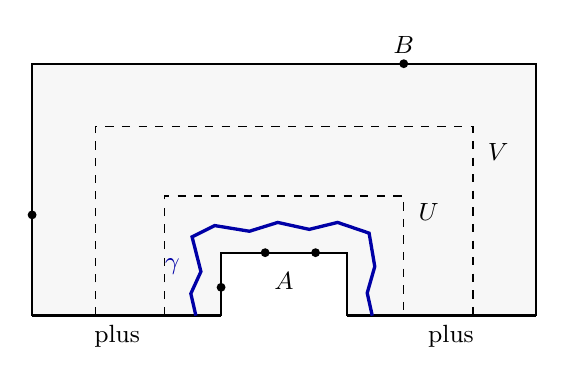
\begin{tikzpicture}[scale=.8, every node/.style={font=\small}]
 \fill[black!3] (-4,0)--(-4,4)--(4,4)--(4,0)--(1,0)--(1,1)
                  --(-1,1)--(-1,0)--cycle;
 \draw[thick] (-4,0)--(-4,4)--(4,4)--(4,0);
 \draw[thick] (-1,0)--(-1,1)--(1,1)--(1,0);
 \draw[very thick] (-4,0)--(-1,0) (1,0)--(4,0);
 \draw[dashed] (-1.9,0)--(-1.9,1.9)--(1.9,1.9)--(1.9,0);
 \draw[dashed] (-3,0)--(-3,3)--(3,3)--(3,0);
 \draw[very thick,blue!65!black]
  (-1.4,0)--(-1.48,.35)--(-1.32,.7)--(-1.46,1.25)
  --(-1.1,1.43)--(-.55,1.34)--(-.1,1.48)--(.4,1.37)
  --(.85,1.48)--(1.35,1.31)--(1.44,.78)--(1.32,.36)--(1.4,0);
 \fill (-1,.45) circle (2pt) (-.3,1) circle (2pt)
       (.5,1) circle (2pt);
 \fill (-4,1.6) circle (2pt) (1.9,4) circle (2pt);
 \node at (0,.55) {$A$};
 \node[above] at (1.9,4) {$B$};
 \node[anchor=west] at (1.98,1.65) {$U$};
 \node[anchor=west] at (3.08,2.6) {$V$};
 \node[blue!65!black,anchor=east] at (-1.5,.78) {$\gamma$};
 \node[below] at (-2.65,0) {plus};
 \node[below] at (2.65,0) {plus};
\end{tikzpicture}
\caption{The dual shell in the free-side argument. The insertion sets
$A,B$ lie at the terminal caps, and $U,V$ are buffered cuts. An open
screen $\gamma$ joins the two plus sides between $A$ and $U$.
Revealing it from the $U$ side leaves the ordinary FK law on its
insertion side, with the screen wired plus. The drawing is schematic.}
\label{fig:boundary-screen}
\end{figure}

We claim the uniform bounds
\begin{equation}
 \|F_A\|_\infty\le C\langle s_A\rangle_*,
 \qquad
 \|F_B\|_\infty\le C\langle s_B\rangle_*.
 \label{eq:buffered-insertion-bound}
\end{equation}
The constant must be independent of the number of insertions.
This is why an absolute correlation estimate alone would not prove
the desired projective bound.

Here is an FK proof of \eqref{eq:buffered-insertion-bound}. For an
insertion set $A$, let $\mathcal E_A$ be the event that every open
cluster not meeting a pinned vertex meets $A$ an even number of times.
With all pins plus, Edwards--Sokal gives
$\langle s_A\rangle=\phi(\mathcal E_A)$. The event
$\mathcal E_A$ is increasing: merging two admissible unpinned clusters
preserves even parity, and joining a cluster to the pins removes its
parity constraint. For arbitrary signs on the cut, the FK edge law
is the law with all pins wired, conditioned on there being no actual
open path between differently signed pins. This follows by counting
the free spin choices of clusters. The conditioning event is
decreasing; paths in this statement use edges of the graph, not the
external wiring. If $m_A^{\mathrm{cut},+}$ denotes the insertion
expectation with the cut pinned plus, Edwards--Sokal and FKG give
\begin{equation}
   |\langle s_A\mid U=u\rangle_*|
       \le\phi_{\mathrm{plus\ cut}}(\mathcal E_A)
       =m_A^{\mathrm{cut},+}.
 \label{eq:insertion-plus-cut}
\end{equation}

To compare this quantity with the uncut expectation, require an open
transverse crossing in a proportional buffer between $A$ and the cut,
joining the two plus-pinned rays. Pure FK-Ising RSW gives this event
probability at least $c>0$, uniformly in exterior boundary conditions
\cite{CDH}. Reveal an outermost such crossing $\gamma$ from the cut
side. This screen separates the insertions from the cut and is connected
to the plus pins. Conditional on the reveal, its insertion side has
the ordinary FK law with $\gamma$ wired plus.

The nearer wired screen increases the parity-event probability, even
for an arbitrarily large insertion set. Indeed restrict the farther
plus-cut law to the region between the terminal and $\gamma$.
Its induced partition is dominated by full wiring on $\gamma$.
The farther-cut parity event implies the near-region parity event
where all clusters touching $\gamma$ are exempt. Since this latter
event is increasing, its probability with $\gamma$ wired is at least
$m_A^{\mathrm{cut},+}$. In the uncut law the revealed screen is actually
connected to the plus rays, so the near-region parity event implies
the full parity event. Hence
\[
 \langle s_A\rangle_*
     \ge c\,m_A^{\mathrm{cut},+}.
\]
Together with \eqref{eq:insertion-plus-cut}, this proves
\eqref{eq:buffered-insertion-bound}; the other cap is identical.
Fixed-shape buffers give the same argument in corner sectors.

The joint law of $U,V$ is a positive left factor, the intervening
pinned-ray kernel, and a positive right factor. If that kernel has
projective diameter $a$, its normalized conditional rows differ by
relative factors in $[e^{-a},e^a]$. Averaging a row over the first
marginal gives
\begin{equation}
 e^{-a}\le
 \frac{\mathbb P(U=u,V=v)}{\mathbb P(U=u)\mathbb P(V=v)}
 \le e^a.
 \label{eq:cut-relative-density}
\end{equation}
For the straight shell we have $a\le Cd^{-2}$. The spin Markov
property makes the two insertion regions conditionally independent
given $U,V$. Thus \eqref{eq:buffered-insertion-bound} and
\eqref{eq:cut-relative-density} imply
\begin{align*}
 \big|\langle s_A s_B\rangle_*
            -\langle s_A\rangle_*\langle s_B\rangle_*\big|
 &\le (e^a-1)\,\mathbb E|F_A(U)|\,\mathbb E|F_B(V)|\\
 &\le C d^{-2}\langle s_A\rangle_*\langle s_B\rangle_*.
\end{align*}
For sufficiently large fixed $d$ this is relative factorization with
error less than $1/2$, uniformly over both insertion sets. Substitution
in \eqref{eq:free-boundary-duality} proves the asserted bound for
$\overline T$. In a corner, choose the fixed ratio large enough that
the pinned-ray diameter is small; the identical argument gives the
finite bound for the free-ray quotient kernel.

\paragraph{A change of boundary condition.}
It remains to bound a shell with one plus ray and one free ray.
Enlarge the terminal groups along both rays as in the pinned case.
The added spins on the free ray may first be conditioned upon and
then summed out; summation preserves the resulting projective bound.
Supermodularity again reduces the problem to the extreme terminal
assignments. The domain-wall expansion used in
\eqref{eq:free-boundary-duality} now has one dual plus ray.
Indeed, after the terminal enlargement the remaining free primal
segment is the same in all four extreme assignments, so its dual
plus ray and its endpoints are unchanged. Reversing a terminal
creates one prescribed wall end where that terminal meets the pinned
primal ray; at its other endpoint walls may end on the free primal
segment without a parity constraint. Thus the terminal assignments
$++,+-,-+,--$ give source sets
$\varnothing,\{y\},\{x\},\{x,y\}$, respectively, in one fixed dual
model. Cancelling the separate terminal factors expresses their
cross ratio as
\begin{equation}
 \frac{\langle s_xs_y\rangle_*}
      {\langle s_x\rangle_*\langle s_y\rangle_*}.
 \label{eq:mixed-boundary-ratio}
\end{equation}
There are just two insertions, at the switches on the pinned primal
ray. Their dual neighborhoods are locally straight and free, and
are a positive distance from each other and from the dual plus ray.
All these distances are fixed proportions of the shell geometry.

Choose disjoint half-box neighborhoods $D_x,D_y$ of these sites,
each with several separated concentric half-boxes inside it. Let
$q_x$ be the probability, in $D_x$ with its artificial outer cut wired,
that $x$ has an actual open arm to a fixed inner radius $\rho_x$.
The true straight boundary remains free. Define $q_y$ likewise.
In the Edwards--Sokal expression for $\langle s_xs_y\rangle_*$,
either the two sites are in the same cluster or both are joined to
the plus pins. Either possibility requires the two local arms.
Conditional on all edges outside one neighborhood, full wiring of
its artificial cut dominates the induced partition. Applying this
bound successively in the two disjoint neighborhoods gives
\begin{equation}
             \langle s_xs_y\rangle_*\le q_xq_y.
 \label{eq:mixed-two-arm-upper}
\end{equation}

We next justify the reverse one-point comparison
\begin{equation}
       \langle s_x\rangle_*\ge c q_x,
       \qquad \langle s_y\rangle_*\ge c q_y.
 \label{eq:mixed-one-arm-lower}
\end{equation}
Choose the nested radii, for example, as
$\rho/2,3\rho/4,\rho,2\rho,3\rho,6\rho$, with the artificial cut
at the last radius. In the uncut model require a transverse open
screen in the half-annular band between $2\rho$ and $3\rho$, and
connect it to the actual plus boundary on its outer side. A fixed
chain of overlapping corridors, together with a radial crossing that
must meet the transverse crossing, realizes these requirements.
RSW and FKG give a positive lower bound independent of the mesh.
Reveal the outermost screen from outside, including its connection
to the plus pins; the reveal does not inspect edges on the inner side.

Inside the screen, full wiring of this nearer cut dominates every
partition induced from the farther wired cut at radius $6\rho$.
Hence the conditional probability of an arm to radius $\rho$ is
at least $q_x$. Extending this arm to the screen costs only another
constant. Indeed require a transverse primal crossing in the smaller
half-annular band between $\rho/2$ and $3\rho/4$ and extend it through
overlapping deterministic corridors to beyond radius $3\rho$.
Every arm from the site to radius $\rho$ meets the transverse crossing.
All these requirements are increasing, so FKG and RSW give their
joint occurrence with the arm at a fixed positive fraction of its
probability. An irregular revealed screen causes no loss: it stays
between the prescribed radii, and a corridor crossing continuing
beyond those radii must first reach it. Equivalently, use free
boundary conditions in a deterministic larger half-box for the
crossing lower bound; the law with the nearer screen wired dominates
on the shared edges, since all exterior attachments meet that wired
cut. This proves \eqref{eq:mixed-one-arm-lower}.

Equations \eqref{eq:mixed-two-arm-upper} and
\eqref{eq:mixed-one-arm-lower} bound \eqref{eq:mixed-boundary-ratio}
above by $c^{-2}$. Griffiths' inequality bounds it below by $1$.
The extreme-comparison reduction therefore gives a finite projective
diameter in the mixed case.

Every use of a continuum limit above involves a fixed finite list of
ratios and straight marked boundary pieces. The corresponding locally
regular approximations include rounded caps and bounded layer shifts.
If uniformity over these approximations failed, a violating sequence
with the same limiting polygon and straight marked pieces would
contradict that convergence theorem. Taking the finest threshold for
the finite list of shapes proves the stated uniformity.
\end{proof}

\subsection{Conditional expectations and positive weights}

The kernel estimate concerns whole spin vectors, rather than individual
spins. It therefore transfers directly to a function of an entire
inner patch. We record also the logarithmic version needed when that
function is a possibly large perturbation of the energy.

\begin{corollary}
\label{cor:boundary-observables}
Let a spin patch of diameter at most $r$ be separated from prescribed
remote spins $\zeta$ by pure shells of one of the types in
Lemma~\ref{lem:boundary-transfer}, out to distance $R=dr$.
Allow fixed proportional buffers around the patch and the outer cut.
Let $H$ be a bounded real function of the patch spins and of any
independent auxiliary variables in the patch. In the free/free case
assume that the region inside the shell has no pinned spins and that
$H$ is invariant under reversal of all its spin arguments.
There are constants $C<\infty$ and $\eta>0$ such that
\begin{align}
 \mathop{\mathrm{osc}}_\zeta\mathbb E_{\mathrm{pure}}[H\mid\zeta]
       &\le C a(d)\|H\|_\infty,
       \label{eq:boundary-expectation-transfer}\\
 \mathop{\mathrm{osc}}_\zeta
        \log\mathbb E_{\mathrm{pure}}[e^H\mid\zeta]
       &\le C a(d)\|H\|_\infty,
       \label{eq:boundary-log-transfer}
\end{align}
where $a(d)=d^{-2}$ at a straight homogeneous side and
$a(d)=d^{-\eta}$ at a corner or boundary-condition change.
Here $\mathop{\mathrm{osc}} f=\sup f-\inf f$. The bounds hold for
each fixed sufficiently large $d$ and sufficiently fine mesh, with
thresholds chosen simultaneously for any finite collection of ratios.
\end{corollary}

\begin{proof}
The spin Markov property factors the conditional law across the two
caps into the shell kernel and positive factors on its two sides.
If the shell diameter is $a$, the conditional distributions on the
inner cap, for any two remote conditions, have relative densities in
$[e^{-a},e^a]$. Their mixtures with the conditional law of the inner
patch have the same comparison. With free rays, spin reversal shows
that the distribution of the patch modulo global sign depends only
on the outer spin vector modulo sign. Thus the quotient kernel gives
precisely this comparison for even functions, even when the remote
spins were specified with absolute signs. Integrating independent
auxiliary variables preserves all the bounds.

At a straight side, \eqref{eq:straight-boundary-transfer} now yields
\eqref{eq:boundary-expectation-transfer}. It also bounds the
oscillation of the logarithm of the expectation of any positive
function by $Cd^{-2}$. To retain the factor $\|H\|_\infty$ when
$\|H\|_\infty\le1$, apply relative-density comparison to $e^H-1$;
its supremum norm is at most $e\|H\|_\infty$, while all expectations
of $e^H$ are at least $e^{-1}$. When $\|H\|_\infty>1$, the direct
projective bound is already at most $Cd^{-2}\|H\|_\infty$.

At a corner or change point, divide the region into $m$ successive
shells of the fixed ratio in Lemma~\ref{lem:boundary-transfer}, with
$m\ge c\log d-C$. A diameter bound $D<\infty$ gives a common
positive fraction $e^{-D}$ in every pair of normalized rows.
Consequently conditional expectation contracts oscillation by at most
$q=1-e^{-D}<1$ through each shell. Composition gives a bound
$Cq^m\|H\|_\infty$, which is \eqref{eq:boundary-expectation-transfer}
for some $\eta>0$. The quotient by sign is preserved at every free
shell.

For \eqref{eq:boundary-log-transfer} with $\|H\|_\infty\le1$,
apply the same contraction to $e^H$ and then use the lower bound
$e^{-1}$. For $\|H\|_\infty>1$, first pass through one shell.
The resulting positive function $h$ satisfies
$\mathop{\mathrm{osc}}\log h\le D$, independently of the size of
$H$. Multiplying $h$ by a constant, arrange $1\le h\le e^D$.
The remaining shells contract its ordinary oscillation to at most
$q^{m-1}(e^D-1)$ and preserve its lower bound $1$. Its logarithmic
oscillation has the same upper bound. Absorbing the first shell into
the constant gives $Cd^{-\eta}\le Cd^{-\eta}\|H\|_\infty$.
This argument uses no exponential moment assumption on $\|H\|_\infty$.
\end{proof}

\section{Partition functions up to a polygon boundary}
\label{sec:polygon}

The bulk scale map controls perturbations whose determining neighborhoods
lie in the plane.  We now extend it to a fixed polygon, integrating all
the way to its boundary.  The additional estimates concern logarithms of
partition functions.  The transfer bounds of Section~\ref{sec:boundary}
make the boundary contributions contract without any cancellation in the
environmental mean.

We formulate the comparison on a flat surface because the later slit
argument will use several copies of portions of the same lattice.  This
does not change the local pure model or introduce independent disorder
on the copies.

\begin{definition}[Polygons on sheets]\label{def:sheet-polygon}
Let $\mathcal S$ be an oriented flat surface with a map
$\pi:\mathcal S\to\R^2$ whose restriction to each sufficiently small
neighborhood is an orientation-preserving isometry.  A \emph{collared
orthogonal polygon} is a compact polygonal disk $\mathcal P\subset
\mathcal S$ such that $\pi$ is defined on a neighborhood of
$\mathcal P$, and each side of $\mathcal P$ is horizontal or vertical in
these local coordinates.  The polygon has finitely many sides; the map
$\pi$ need not be injective on $\mathcal P$.

Its lattice approximation is obtained by rounding its sides to the
lifted square grid of mesh $\delta$ and filling the resulting polygon.
Boundary-condition changes are placed in straight side interiors and
rounded with the sides.  Distinct lifted copies of a physical lattice
edge are distinct random-cluster edges with the same environmental
sign.  Thus the coupling of a lifted edge $\widetilde e$ is the coupling
of $\pi(\widetilde e)$.
\end{definition}

The ordinary plane case is included.  A collar permits small changes
of sides and marked positions without changing the local charts.  All
lattice conventions below allow a bounded number of boundary layers;
the rounding prescription is fixed for each test.

\begin{proposition}[Fixed polygon comparison]
\label{prop:polygon-comparison}
There exists $\theta_0>0$ with the following property.  Fix
$0<\theta<\theta_0$, a collared orthogonal polygon $\mathcal P$, and
four distinct boundary marks in straight side interiors.  Wire each of
two opposite marked boundary arcs separately and leave the intervening
arcs free.  On the rounded lifted grid assign odds
\[
 v_e=\sqrt2\exp(\theta\xi_e),
\]
where the physical-edge signs are independent and symmetric, and
repeated lifted edges have the same sign.  Let $\phi_{\delta,J}^{\rm sep}$
and $\phi_{\delta,0}^{\rm sep}$ denote respectively this random-cluster
law and the pure law on the same graph and with the same boundary
partition.  If $\mathcal A_\delta$ is the event of an actual open path
between the two wired arcs, then
\begin{equation}\label{eq:polygon-comparison}
 \phi_{\delta,J}^{\rm sep}(\mathcal A_\delta)
 -\phi_{\delta,0}^{\rm sep}(\mathcal A_\delta)
 \longrightarrow0
 \qquad\text{in environmental probability as }\delta\downarrow0.
\end{equation}
The disorder threshold is independent of the fixed polygon and marks.
The conclusion also holds on the dual square grid.
\end{proposition}

For the proof, constrain the spin to be constant on each wired arc.
Write $\mathcal Z_J^{++}$ and $\mathcal Z_J^{+-}$ for the two partition
functions obtained by fixing these constants, with free spins on the
remaining boundary arcs.  The Edwards--Sokal correspondence gives
\begin{equation}\label{eq:polygon-spin-ratio}
 \phi_{\delta,J}^{\rm sep}(\mathcal A_\delta)
 =\frac{\mathcal Z_J^{++}-\mathcal Z_J^{+-}}
        {\mathcal Z_J^{++}+\mathcal Z_J^{+-}}
 =\tanh\!\left(\frac12\log
                 \frac{\mathcal Z_J^{++}}{\mathcal Z_J^{+-}}\right).
\end{equation}
Indeed, after summing the two possible signs of each arc, their spin
correlation is the probability that their FK clusters are actually
connected.  Global spin flip identifies the other two partition
functions with these two.  We shall compare $\mathcal Z_J^\eta$ with its
pure counterpart $\mathcal Z_0^\eta$, for $\eta\in\{++, +-\}$, while
removing exactly the same scalar factor from both.

\subsection{The scale map with the boundary present}

We first describe the finite-volume implementation sufficiently
explicitly to keep track of that common factor.  Throughout, the norm
of a potential is its supremum over all its spin and reference-variable
arguments.  Independent priorities and thresholds used to construct the
map belong to the environment over which $\E$ averages.  The fair
comparison coins described below are instead Gibbs-field variables,
with an independent product reference law.  We write $\E_0^\eta$ for
pure Ising expectation with pin assignment $\eta$, together with all
these reference variables.

Write $C=C_{\rm s}$ for the fixed support and dependence constant of
Proposition~\ref{prop:bulk-input}, as supplied by the local scale map in
\cite[Section~``An exact local change of scale'']{Q}.  The coarse
spacings are $s_k=s_0L^k$ in lattice units, with $L$ a sufficiently large
odd integer.  All support, allocation, and status-check radii are fixed
multiples of the current spacing.  Their constants can be fixed before
$L$ is chosen.  Choose a positive physical scale $\alpha$, depending
on the polygon, so small that every full determining neighborhood
through scales $\delta s\le\alpha$ lies in an ordinary injectively
projected chart.  If it meets the polygon boundary, it sees at most a
straight side, one corner, or one boundary-condition change.  This is
possible because there are finitely many sides and distinct changes,
and because the closed polygon has a collar.  At a corner whose two
incident rays are pinned, both rays carry the same sign.

For sufficiently small $\delta$, we stop at the largest $N=N(\delta)$ for which
$\delta s_N\le\alpha$.  In particular,
\begin{equation}\label{eq:polygon-terminal-scale}
 \alpha/L<\delta s_N\le\alpha,
 \qquad N(\delta)\longrightarrow\infty.
\end{equation}
The choice of $\alpha$ includes all enlarged neighborhoods used below,
not just the supports of the potentials.  A fixed exterior pad contains
the necessary grid cells and reference variables.  There are no spins
to integrate outside the polygon.  The total overhang accumulated up to
scale $s_N$ is at most a fixed multiple of $s_N$, since the spacings
form a geometric progression.  Consequently an outer truncation beyond
this pad has no effect on any nonzero potential.

Cell indices distinguish different lifts even when their projected
centers coincide.  Within any ordinary chart we use the integer
coordinates of the projected grid.  At spacing $s$, let $f_i$ be the current child potentials and let
$\mathcal C_j$ be the $L^2$ children of the parent at spacing $s'=Ls$.
Set
\[
 \mathcal C_j=Lj+\{-(L-1)/2,\ldots,(L-1)/2\}^2,
 \qquad F_j=\sum_{i\in\mathcal C_j}f_i,
\]
\[
 I_j=\{x:\norm{x-s'j}_\infty<4s'\}.
\]
Coordinates in this display are the ordinary chart coordinates.
Integrating $I_j$ means integrating the free polygon spins and old
reference variables lying there.  The support of $F_j$ lies well inside
$I_j$.

Here is the regular operation of~\cite{Q}.  Fix a numerical range
$D_0=100$ and attach a fair reference coin to every pair of distinct
parents at sup-norm distance at most $D_0$ in parent units.  A parent is
selected when every incident coin favors it. The incident comparisons
form its \emph{comparison star}. Let $A_j$ be its selection
indicator and
\[
 p_{\rm sel}=\E_{\rm ref}A_j=2^{-((2D_0+1)^2-1)}.
\]
Thus $p_{\rm sel}>0$ is fixed independently of $L$, and distinct selected squares
are separated.  Order comparisons by length and then by independent
continuous priorities.  For a comparison edge $e$, let $d_eA_j$ be the
Doob difference obtained by revealing its coin under the reference
law.  This is a local function of the star at $j$: it vanishes if an
earlier comparison has already disfavored $j$.

For fixed old field variables, decorate the new coins successively by
normalized likelihoods
\begin{equation}\label{eq:polygon-decoration}
 \frac{e^{U_e}}{\E_e e^{U_e}},
 \qquad U_e=p_{\rm sel}^{-1}\sum_j F_jd_eA_j,
\end{equation}
where $\E_e$ averages the current fair coin, holding previously revealed
coins fixed.  Since each likelihood is normalized, the decoration
preserves the old field marginal. Only finitely many likelihoods are
nontrivial in this padded finite construction; the plane array is used
to specify their local formulas. The identity
$\sum_e d_eA_j=A_j-p_{\rm sel}$ gives
\begin{equation}\label{eq:polygon-decoration-identity}
 \sum_jF_j+\sum_e\bigl(U_e-\log\E_e e^{U_e}\bigr)
 =p_{\rm sel}^{-1}\sum_j A_jF_j-\sum_e\log\E_e e^{U_e}.
\end{equation}
Every comparison star affecting a nonzero term is retained in full,
including in the exterior pad.  In particular, a normalizer whose old-field support meets an
updated square remains in the expression being integrated.

Given the coins, each normalizer on the right of
\eqref{eq:polygon-decoration-identity} meets at most one selected
square. This is the local separation property of
\cite[Lemma~3.1, \emph{Separation of the terms to be integrated}]{Q}.
Its argument is exactly local: if the endpoint
neighborhoods of a comparison could meet two selected squares, then
for a short comparison the selected centers would be too close; for a
long comparison an endpoint has already lost its shorter comparison
with the nearby selected center.  Its Doob difference is then zero.
The same assertion holds for each selected $F_j$.  If $H_j$ is the sum
of all terms meeting a selected $I_j$, replace it by
\begin{equation}\label{eq:polygon-conditional-addition}
 \log\E_0^\eta[e^{H_j}\mid I_j^c].
\end{equation}
The notation $I_j^c$ includes all unintegrated spins and old reference
variables; the new coins are held fixed.  Pure conditional laws in the
selected squares are independent given their exterior, also when a
square intersects the polygon boundary.  Thus these replacements
preserve the integrated weight exactly.  They leave all old variables
in the field, with pure conditional law in each updated square.

Large potentials are handled by the real-valued modification of the
same map.  Attach to each child an independent environmental threshold
uniform on $[b_0,2b_0]$, and call the child a flag if its norm exceeds
that threshold.  A parent within $10D_0$ parent units of a flag is
inactive.  Set its $F_j$ to zero in~\eqref{eq:polygon-decoration}, retain
its child terms separately, and keep its comparison coins in the full
stars.  Every retained term that touches an active selected square is
included in that square's integration.  Its small support prevents it
from touching two such squares.

Put $d_0=4C+10$.  An isolated group is a nonempty group $A$ of flags of
child-grid diameter at most $6d_0$, with no other flag within $100D_0$
parent units of $A$.  Choose a representative by independent
priorities, let $j(A)$ be its parent, and set
\[
 G_A=\sum_{\operatorname{dist}(i,A)\le3d_0}f_i,
 \qquad I_A=I_{j(A)}.
\]
For large $L$, $G_A$ is supported deep inside $I_A$.  The inactive region
keeps all active integrations and nonzero active coin normalizers away
from $I_A$.  Let $B_A$ be the sum of the remaining terms touching $I_A$.
Replace $G_A$, retaining $B_A$, by
\begin{equation}\label{eq:polygon-isolated-ratio}
 R_A=\log\E_0^\eta[e^{B_A+G_A}\mid I_A^c]
       -\log\E_0^\eta[e^{B_A}\mid I_A^c].
\end{equation}
The isolated groups are separated.  The identity
\begin{equation}\label{eq:polygon-isolated-exactness}
 \E_0^\eta[e^{B_A+R_A}\mid I_A^c]
 =\E_0^\eta[e^{B_A+G_A}\mid I_A^c]
\end{equation}
shows why the background $B_A$ must be kept in this exact operation.
Its removal will be used only in estimating the norm.  Allocate each
integrated term to its integration parent, allocate retained terms to
their parents, and split the remaining pair terms between their
endpoints, as in the fixed local rules of~\cite{Q}.

We next specify the scalar subtractions.  Fix $B$ larger than all the
support and determining-range constants, in parent units, and call a
cell at spacing $s$ a boundary cell if its center is within $Bs$ of the
polygon boundary.  The constant $B$ is fixed before $L$.  At every
scale, including the initial one, use the full-plane pure centering
from~\cite{Q} outside the boundary cells.  For a boundary-cell potential
in the $++$ construction, subtract its $\E_0^{++}$ expectation.  Subtract
that same scalar from the corresponding potential in the $+-$
construction.

\begin{lemma}[Exact boundary implementation]
\label{lem:boundary-exactness}
For the terminal scale chosen above, the local construction is exact
for each fixed environment and realization of its priorities and
thresholds.  Its potentials have support and environmental dependence
radius at most $Cs_k$.  Outside the
boundary cells they are the plane potentials, or zero outside the pad.
The two pin assignments admit the same scalar subtractions.  More
precisely, there is a scalar $a_\delta$, independent of the pin
assignment, such that
\begin{equation}\label{eq:polygon-exact-partition}
 \frac{\mathcal Z_J^\eta}{\mathcal Z_0^\eta}
 =e^{a_\delta}\E_0^\eta
       \exp\!\left(\sum_i f_i^{(N),\eta}\right),
 \qquad \eta\in\{++, +-\}.
\end{equation}
The initial boundary norms are uniformly $O_{s_0}(\theta)$.
\end{lemma}

\begin{proof}
Allocate the initial bond perturbations as in
\cite[Section~``Tuning a trajectory with vanishing perturbations'']{Q},
using only bonds present in the polygon.  A cell receives the allocated
terms $(K_e-K_0)\sigma_x\sigma_y$, followed by the specified centering.
For fixed $s_0$ there are boundedly many such terms per cell, and
$|K_e-K_0|=O(\theta)$; this proves the initial bound.  Subtracting
constants changes only the scalar partition factor.

The identities \eqref{eq:polygon-decoration-identity},
\eqref{eq:polygon-conditional-addition}, and
\eqref{eq:polygon-isolated-exactness} prove exactness at each step.
They hold for every conditional pure probability kernel; the presence
of the boundary merely reduces the set of spins integrated in a
square.  The allocation and status checks use the same finite stencils
as in the plane.  The choice of $C$ in the local map already covers
these stencils and the $C/L$ overhang from the child scale.  Restricting
the pure integrations to polygon spins does not enlarge either radius.
This proves locality.  Choosing
$B$ with slack so that $B>C_1+B/L$, where $C_1$ bounds the complete
parent determining radius, shows inductively that every input of a
nonboundary output is also nonboundary.  There the construction is
precisely the plane construction.  The pad similarly contains all
possibly nonzero outputs.

Every determining neighborhood sees at most one local pin sign.
Spin flip commutes with the conditional integrals, and with every
algebraic operation in the decoration and the isolated ratio.  Hence
changing that sign conjugates the local potential by simultaneous
flip of its spin and pin arguments.  The corresponding norms agree;
using the same thresholds and priorities therefore gives the same
flags, isolation decisions, and local scalar subtraction.  If no pin
lies in a determining neighborhood, its potential is spin-flip even.
The constants used for boundary centering are deterministic
functionals of the local potential: dependence on the fixed pure
polygon does not introduce dependence on remote random bonds.

In particular the $+-$ potentials need not be centered for the pure
$+-$ expectation.  Exactness only requires that the subtracted
constants agree between the two constructions.  Iterating the exact
identities with those constants gives
\eqref{eq:polygon-exact-partition}.
\end{proof}

\subsection{Contraction of the boundary potentials}

Let $X_k$ be the root moment of the plane potentials supplied by
Proposition~\ref{prop:bulk-input}, with its fixed order $P>2$, and let
\begin{equation}\label{eq:polygon-boundary-moment}
 Z_k=\max_{i\text{ a boundary cell}}
       \bigl(\E\norm{f_i^{(k),++}}_\infty^P\bigr)^{1/P}.
\end{equation}
The maximum is zero if there are no boundary cells.  By local spin-flip
conjugacy the same quantity bounds the $+-$ construction.  We take the
maximum of the individual moments, rather than the moment of a maximum.
No stationarity along the polygon boundary is required.

\begin{lemma}[Boundary recurrence]\label{lem:boundary-recursion}
The scale-step parameters can be chosen in the order: $L$ sufficiently
large, $b_0$ sufficiently small, and $s_0$ sufficiently large, so that
for all $k<N$,
\begin{equation}\label{eq:boundary-recurrence}
 Z_{k+1}\le q_* Z_k+C_LX_k
                    +C_{L,b_0}(Z_k+X_k)^2,
 \qquad q_*<1.
\end{equation}
The constants are independent of the polygon and the mesh, provided
the determining neighborhoods have the boundary geometries and chart
properties specified above.  For sufficiently small $\theta$, the
boundary moments remain uniformly small and tend to zero as the
scale index tends to infinity, uniformly over all the finite runs.
\end{lemma}

\begin{proof}
There are four contributions to the recurrence.  The linear transfer
of boundary logs contracts by the summable side estimate; unflagged
Taylor remainders are small because their input norms are at most
$2b_0$.  On flagged stencils, a distant independent flag gives an
extra moment factor.  The remaining dependent logs form an isolated
group, to which the positive-weight transfer estimate applies.
Bulk inputs in each case are bounded by a constant times $X_k$.

We first estimate the linearized regular map.  Its plane formula from
\cite[Lemma~3.2, \emph{Regular linearization}]{Q} remains valid before the
specified output centering:
\[
 p_{\rm sel}^{-1}A_j\sum_{i\in\mathcal C_j}
          \E_0^{++}[f_i\mid I_j^c].
\]
The derivative of each coin normalizer is zero, and the derivative of
a conditional log integral is conditional expectation.  For a
boundary child the pure mean is zero, so its transferred supremum is
bounded by its oscillation.  The reference variables in its patch are
integrated with their pure product law.  The same bound for the other
pin assignment follows by the local flip described in
Lemma~\ref{lem:boundary-exactness}.

We claim that the sum of the transfer coefficients over boundary
children in one determining stencil is $o_L(1)$.  Distances in the next
paragraph are measured in child units.  All these cells lie in a strip
of fixed width $B$ along a side.  If a cell is within a fixed distance
of a corner or a change, choose an inner sector shell containing its
whole support and determining patch.  The corner or change estimate
of Lemma~\ref{lem:boundary-transfer}, composed to a radius proportional
to $L$, makes its transfer coefficient tend to zero as $L$ grows.
All those shells fit inside the parent integration square with room
to condition onward.

For the remaining cells let $t$ be their distance along the side to
the nearest corner or change, capped at $L$; in a neighborhood without
a feature set $t=L$.  Once $t$ exceeds a fixed support-dependent
constant, a straight half-shell reaches a radius proportional to $t$
without seeing a different boundary condition.  Its coefficient is
at most $C't^{-2}$ by Lemma~\ref{lem:boundary-transfer}.  On a free side
the full determining stencil avoids pins, so the potential is even,
as required by that lemma.  There are $O(t)$ boundary cells in each
dyadic range $[t,2t]$, including $O(L)$ in the last capped range.
Consequently, for any sufficiently large fixed $t_0$,
\begin{equation}\label{eq:boundary-summable-transfer}
 \sum_i a_{i,L}
 \le \sum_{t_i\le t_0}a_{i,L}+\frac{C''}{t_0},
 \qquad
 \lim_{L\to\infty}a_{i,L}=0
       \quad\text{for each member of the first, bounded list}.
\end{equation}
First choosing $t_0$ and then $L$ proves the claim.  The same calculation
holds for a fixed enlargement of the child patches or the boundary
strip.  Patches with no free spins cause no difficulty, since only
their reference variables remain to be integrated.

Multiplication by $A_j/p_{\rm sel}$ costs at most $p_{\rm sel}^{-1}$, which is independent
of $L$, and output centering costs at most a factor two.  Minkowski's
inequality and \eqref{eq:boundary-summable-transfer} therefore bound
the boundary-child part of the linearized output by $o_L(1)Z_k$.
All bulk inputs can be bounded crudely, giving $C_LX_k$.
Only finitely many fixed shell ratios are needed once $L$ is fixed;
we subsequently choose $s_0$ large enough for all their pure estimates.

It remains to control the actual map in the $P$th moment.  Set
$X=Z_k+X_k$.  Every child norm in an enlarged determining stencil has
root moment at most $X$.  On a stencil without flags, every child norm
is at most $2b_0$.  Conditional integrations are probability kernels,
so the regular map has uniform Taylor bounds after $L$ is fixed.
Writing $S$ for the sum of its child norms, its remainder is bounded
by $C_LS^2\le C_Lb_0S$.  Its root-moment cost is thus $C_Lb_0X$.
The real map, without any smallness restriction, has the crude bound
$C_LS$ by $|\log\E_0e^H|\le\norm{H}_\infty$ and the analogous
Lipschitz bound for differences of such logarithms.

Small flag probability alone would not improve this last estimate in
the $P$th moment.  We use the location of the flags, as in
\cite[Section~``The contribution of isolated large terms'']{Q}.
Enlarge the determining stencil to include all isolation checks and
all child neighborhoods of radius $100D_0L+2C$ about a contributing
child.  If a flag $h$ in this enlarged stencil is farther than $2C$
child units from a charged child $i$, their environmental dependence
neighborhoods are disjoint.  Its fresh threshold is independent too,
and Markov's inequality gives
$\P(h\text{ is a flag})\le b_0^{-P}X^P$.  Hence
\begin{equation}\label{eq:boundary-independent-flag}
 \E\!\left[\norm{f_i}_\infty^P
                    {\bf1}_{\{h\text{ is a flag}\}}\right]
 =\E\norm{f_i}_\infty^P\,
       \P(h\text{ is a flag})
 \le C_{b_0}X^{2P}.
\end{equation}
There are only finitely many charges for fixed $L$, so these
contributions cost $C_{L,b_0}X^2$ in root moment.

If no such independent flag is available for a contributing term,
every relevant flag lies within $2C$ of that term.  These flags form
one bounded child-radius group.  The enlarged stencil contains the
whole isolation neighborhood, so either they are an isolated group
of the construction, or a farther flag is present and
\eqref{eq:boundary-independent-flag} applies.  In the isolated case,
all logs possibly dependent on the triggering flags are included in
$G_A$.  For every probability kernel $P_0$,
\begin{equation}\label{eq:boundary-remove-background}
 \left|\log\frac{P_0e^{B_A+G_A}}{P_0e^{B_A}}
                    -\log P_0e^{G_A}\right|
 \le2\norm{B_A}_\infty.
\end{equation}
Each child in $B_A$ is outside the concentration neighborhood and is
independent of an actual triggering flag.  Its occurrence can again be
charged using \eqref{eq:boundary-independent-flag}.  The same applies
to every term omitted from the concentrated contribution.

After this estimate, the only remaining large term to bound is the
centered form of
\[
 \log\E_0^{++}[e^{G_A}\mid I_A^c].
\]
Corollary~\ref{cor:boundary-observables} applies to this positive
weight for any size of $\norm{G_A}_\infty$.  A group containing a
boundary child has bounded child diameter.  There are boundedly many
possible flag patterns at each anchor and boundedly many logs in each
concentration neighborhood, with bounds independent of $L$.
Thus its logs all lie in
a fixed enlargement of the boundary strip, and the shell coefficient
at its anchor multiplies the sum of their norms.  Summing over all
possible boundary anchors gives the same arbitrarily small sum as in
\eqref{eq:boundary-summable-transfer}.  We may sum before taking the
root moment by Minkowski's inequality; neither a supremum over anchors
nor independence among their events is needed.  Groups containing
only bulk inputs contribute at most $C_LX_k$ by the crude bound.
The linearized terms restricted to flagged stencils, if subtracted in
comparing the two maps, obey the identical dichotomy: either charge
them to an independent flag or use the linear shell transfer for the
bounded local group.

Combining these estimates gives
\[
 Z_{k+1}\le
  \bigl(o_L(1)+C_Lb_0\bigr)Z_k+C_L'X_k
                   +C_{L,b_0}(Z_k+X_k)^2.
\]
Choose $L$ so the first term leaves a strict contraction margin, then
choose $b_0$ within that margin, and finally choose $s_0$ for the
finite list of pure shell estimates.  These choices are compatible
with the parameter freedoms in Proposition~\ref{prop:bulk-input}.
This proves \eqref{eq:boundary-recurrence}.

For completeness, take a deterministic scalar majorant for all the
finite polygon runs, starting from their uniform $O_{s_0}(\theta)$
bound and iterating the right side of
\eqref{eq:boundary-recurrence}.  Choose a small invariant interval so
that the quadratic term has Lipschitz constant less than half the
remaining contraction margin.  Proposition~\ref{prop:bulk-input}
makes $\sup_kX_k$ as small as required by decreasing $\theta$; the
initial majorant is small by the same choice.  The majorant therefore
stays in that interval.  Since $X_k\to0$, its limsup $z$ satisfies
$z\le q_*z+C_{L,b_0}z^2$, which forces $z=0$ in the chosen interval.
This proves uniform smallness and decay.
\end{proof}

\subsection{Completion of the partition comparison}

\begin{proof}[Proof of Proposition~\ref{prop:polygon-comparison}]
All determining stencils used in Lemma~\ref{lem:boundary-recursion}
lie in ordinary injectively projected charts.  The physical-edge
signs within each such stencil have their usual iid law.  In
particular, disjoint dependence neighborhoods used in
\eqref{eq:boundary-independent-flag} are genuinely independent.
There is no requirement of independence between different sheets:
the entire enlarged stencil, including its overhang, was placed in
one ordinary chart before the terminal scale was selected.

By \eqref{eq:polygon-terminal-scale}, the number of possibly nonzero
terminal potentials, including those in the pad, is bounded for this
fixed polygon.  This bound may depend on its geometry and on
$\alpha$, but not on the mesh.  Proposition~\ref{prop:bulk-input} and
Lemma~\ref{lem:boundary-recursion} therefore give
\[
 S_\delta=\sum_i\max_{\eta\in\{++, +-\}}
                 \norm{f_i^{(N),\eta}}_\infty
 \longrightarrow0
 \quad\text{in }L^1\text{ of the environment and construction choices}.
\]
Applying \eqref{eq:polygon-exact-partition} yields
\[
 \left|\log\frac{\mathcal Z_J^\eta}{\mathcal Z_0^\eta}
                      -a_\delta\right|\le S_\delta,
 \qquad \eta\in\{++, +-\}.
\]
The common scalar cancels from the difference.  Since $\tanh$ is
Lipschitz, \eqref{eq:polygon-spin-ratio} proves the comparison with an
error bounded by $S_\delta$.  The partition ratios themselves do not
depend on the construction choices.  Averaging the bound over those
choices thus gives convergence in environmental probability alone.

The local boundary shapes are the straight side, the two orthogonal
corner angles, and a single fixed/free change.  Their constants, and
all scale-map parameters, were chosen independently of the polygon;
only the positive terminal physical scale depended on it.  This
proves the asserted uniform disorder threshold.  On the dual grid,
duality replaces $v_e$ by $2/v_e$, hence $\theta\xi_e$ by
$-\theta\xi_e$.  This has the same environmental law, and the same
argument applies.
\end{proof}

\section{Four marked boundary points and the exploration drawing}\label{sec:pure}

Proposition~\ref{prop:polygon-comparison} compares the random model with
the pure model on the same finite graph. We now identify the pure limit
and specify the finite exploration laws that will be used after stopping.
The distinction between an actual FK crossing and an interface pairing is
important: deterministic boundary closures give the two events different
relative weights.

\subsection{Pairings and boundary closures}

At each lattice edge, the medial representation has a tile with four
ports and two noncrossing pairings of those ports. The open state joins
the two primal corners; the other state joins the dual corners.
Joining the ports of adjacent tiles gives loops and, at marked boundary
changes, open strands. Give an open switch local weight $v_e/\sqrt2$
and a closed switch weight $1$. The \emph{open-cap law} assigns a
configuration weight equal to the product of its local switch weights
times $(\sqrt2)^{\ell}$, where $\ell$ is the number of internal closed
loops. Open strands receive no extra factor. At the pure critical odds
$v_e=\sqrt2$, the two local weights are equal.

Label the four ports in cyclic order by $a,b,c,d$, with designated
primal arcs $ab$ and $cd$. There are two noncrossing pairings:
$E_{\mathrm P}=\{a\leftrightarrow d,\ b\leftrightarrow c\}$ and
$E_{\mathrm D}=\{a\leftrightarrow b,\ c\leftrightarrow d\}$.
Under separate primal closure, $E_{\mathrm P}$ is exactly the event of
an actual primal crossing; under separate dual closure,
$E_{\mathrm D}$ is the analogous dual event.

A four-change exploration also specifies a distinguished starting
port and follows the unique strand issuing from that port until it
reaches another marked port. This choice is part of the experiment,
independent of the cyclic labels used for the electrodes. In the
short-interval experiment of Section~\ref{sec:identification}, the
chosen port is the original chordal starting point.

This is a finite measure defined by the loop representation. It need not
be identified with a boundary partition of the original primal graph.
The following exact change of measure supplies the connection.

\begin{lemma}[Cap change]\label{lem:cap-change}
Let $p$ be the probability of $E_{\mathrm P}$ in a four-change open-cap
law with arbitrary positive FK edge odds. Under separate primal closure,
the probability of an actual primal crossing is
\begin{equation}\label{eq:cap-change}
 \mathcal G(p)=\frac{p}{p+\sqrt2(1-p)}.
\end{equation}
The same formula holds for conditional probabilities after any exploration
history that reveals only encountered switches. The density between the
two full-configuration laws and its reciprocal are bounded by absolute
constants. The analogous statement holds with primal and dual interchanged.
\end{lemma}

\begin{proof}
Fix the internal switches. The two possible boundary pairings acquire
numbers of additional loops differing by one under separate primal
closure. The noncrossing outcome acquires the extra factor $\sqrt2$.
The local edge factors are unchanged. Thus the separate-closure law has
density proportional to
$\ind_{E_{\mathrm P}}+\sqrt2\ind_{E_{\mathrm D}}$
relative to the open-cap law. Normalization proves
\eqref{eq:cap-change} and the density bounds. Conditioning this same
two-valued density on the full revealed history proves the conditional
identity. In particular, no Markov property of a putative limiting curve
is being used. This is the finite cap calculation of~\cite[Section
``Alternating tests after exploration'']{C}; it does not require constant
edge odds.
\end{proof}

\subsection{The pure four-point limit on a flat disk}

For a marked conformal disk $(P;a,b,c,d)$, let $\psi:P\to\Hh$ send
$(a,c,d)$ to $(0,1,\infty)$ and put $\chi=\psi(b)\in(0,1)$.
The primal electrodes are $ab$ and $cd$. With the convention above,
$E_{\mathrm P}$ is rare when $\chi\downarrow0$. Define
\begin{equation}\label{eq:four-point-functions}
 \begin{split}
 f(\chi)&=
 \frac{\sqrt{1-\sqrt{1-\chi}}}
 {\sqrt{1-\sqrt\chi}+\sqrt{1-\sqrt{1-\chi}}},\\
 g(\chi)&=\frac{f(\chi)}{f(\chi)+\sqrt2(1-f(\chi))}.
 \end{split}
\end{equation}
The function $f$ is the pure open-cap pairing probability; $g$ is the
actual crossing probability under separate primal wiring. The
normalization agrees with the $q=2$ specialization in~\cite[Proposition
``Jordan-quad transfer'']{C}. In the convention of
\cite[Equation~(1.1)]{CS}, setting $u=1-\chi$ gives the complementary
pairing probability $1-f(\chi)$. This accounts for the apparent reversal
of the small-interval limit between the two conventions. In particular,
\begin{equation}\label{eq:four-point-properties}
 f(1-\chi)=1-f(\chi),\qquad
 f(\chi)\sim\sqrt{\chi/2}\quad(\chi\downarrow0).
\end{equation}
Both functions are continuous on $[0,1]$ and smooth in its interior.

\begin{proposition}[Pure four-point limit]\label{prop:pure-four-mark}
Let $P$ be a fixed collared orthogonal polygon that is a topological disk
in an oriented flat surface with a locally injective translation projection
to the plane. Put four distinct marks in straight boundary portions.
Approximate $P$ by its lifted square grid at mesh $\delta\downarrow0$,
with critical odds $\sqrt2$ on every edge. Then the open-cap probability
of $E_{\mathrm P}$ tends to $f(\chi_P)$, and the probability of an actual
crossing between separately wired arcs $ab$ and $cd$ tends to $g(\chi_P)$.
The conclusion also holds for compatible medial approximations differing
by an incident boundary layer.
\end{proposition}

\begin{proof}
For a planar polygon this is the four-mark observable theorem of
Chelkak--Smirnov~\cite[Theorem~6.1]{CS}, with boundary pairings and
deterministic closures converted as in Lemma~\ref{lem:cap-change}.
We explain why its proof applies to $P$. This is necessary because the
projection of $P$ need not be injective.

\emph{The finite observable.}
The construction combines the two Dobrushin observables obtained by
joining $c$ to $d$, or $a$ to $d$, with a deterministic exterior arc. Its local
s-holomorphic identities and its relation to the two pairing weights
are identities on tiles. The primitive of its square is single-valued
on the disk and is constant on each of the four boundary arcs. In
cyclic order its normalized boundary values are
$0,1,\kappa_\delta,\kappa_\delta$. If
$p_\delta=\P_{\mathrm{open}}(E_{\mathrm P})$, the exact relation is
\begin{equation}\label{eq:primitive-parameter}
 \kappa_\delta=
 \left(\frac{t_\delta^2+\sqrt2t_\delta}
 {t_\delta^2+\sqrt2t_\delta+1}\right)^2,
 \qquad t_\delta=\frac{1-p_\delta}{p_\delta}.
\end{equation}
This extends continuously to $p_\delta=0,1$ and is one-to-one.
It is the normalization in~\cite[Equations~(6.1)--(6.6)]{CS}, with
their pairing probability equal to $1-p_\delta$.

The phases can be computed in the frame supplied by the projection.
A simple closed curve bounding a disk in this flat surface has total
turning $2\pi$ by Gauss--Bonnet. Closing an observable path by a boundary
arc therefore gives the same phase relations as in the plane.
The collar accommodates the deterministic closing arcs. There is no
additional period for the primitive or ambiguity in the half-differential
on a simply connected polygon.

\emph{Compactness and boundary values.}
The bounds on the primitive use its boundary values, the local boundary
modification by half-rhombi, and the discrete maximum principle.
They do not require a global injective coordinate. Interior estimates
for the observable and its primitive apply in ordinary projection
charts. A finite chart cover of each compact subset consequently gives
subsequential convergence to a bounded harmonic primitive $H$ whose
complex differential has the corresponding holomorphic square root.

The constant data and one-sided normal conditions pass to the limit
near open straight sides by the same boundary estimates. In each such
chart, comparison with distant boundary data first stops at the boundary
of a small chart neighborhood; the comparison function there is bounded.
Its contribution near the side is then suppressed by ordinary planar
discrete harmonic measure. Corners have ordinary wedge charts. Their
isolated values do not affect the bounded harmonic Dirichlet problem.
The marked points lie in straight portions, so their two one-sided
conditions are handled in disjoint neighborhoods in the same way.

\emph{Identification of the remaining constant.}
The sign condition needed here is concrete. Denote the two auxiliary
primitives by $H_\delta^\bullet$ and $H_\delta^\circ$, on the black
and white graphs of the observable construction, respectively. The
black primitive is subharmonic and the white one superharmonic;
these color names follow~\cite{CS}. On the arc $cd$,
$H_\delta^\bullet$ at an inward neighbor is at least its boundary
value $\kappa_\delta$. On $da$, $H_\delta^\circ$ has the reversed inequality.
These follow from the observable's boundary tangent condition and the
half-face modification in~\cite[Section~6]{CS}.

To see that these conditions survive in the required sense, suppose
that a limiting harmonic primitive satisfies $H<\kappa$ on a small
interior contour $\mathcal C$ whose endpoints lie in a straight
subinterval of $cd$. Enclose the region between this contour and the
subinterval, entirely within one chart. Let $V_\delta$ be the discrete
harmonic measure of a smaller subinterval strictly between the endpoints.
It vanishes on the contour. Discrete Green's formula and the inward
inequality give
\begin{equation}\label{eq:local-boundary-sign}
 \sum_{u\in\mathcal C_\delta}
       V_\delta(u_{\rm in})
       \bigl(H_\delta^\bullet(u)-\kappa_\delta\bigr)w_u\ge0,
\end{equation}
where $u_{\rm in}$ is the inward neighbor and $w_u>0$ is the local
conductance; multiple boundary incidences are summed separately.
On a fixed middle portion, $V_\delta(u_{\rm in})\ge c_1\delta$ and
there are order $\delta^{-1}$ incidences. Compact convergence thus
bounds that portion of the sum above by a fixed negative number $-c$.
At distance $r$ from an endpoint, the local harmonic-measure bound is
$V_\delta(u_{\rm in})\le C\delta r^{\eta-1}$ for some $\eta>0$.
Summing over the endpoint portions of length $\mu$, and using the
bounded primitive, gives a contribution at most $C\mu^\eta$.
The remaining compact portion has nonpositive contribution for small
mesh. Thus \eqref{eq:local-boundary-sign}
would imply $0\le-c+C\mu^\eta$, a contradiction for small $\mu$.
The dual argument excludes $H>\kappa$ near a subinterval of $da$.
This is exactly the local comparison in
\cite[Equations~(6.8)--(6.10)]{CS}; all its objects lie in one chart.

Pull the limiting boundary-value problem to a conformal disk.
For $0<\kappa<1$ its solution is the imaginary part of a conformal
map to a horizontal strip of height one with a slit at height $\kappa$,
sending $a$ to the lower left end, $b$ to the right end, and $c$ to the
upper left end. If $d$ mapped to the lower slit bank rather than the
tip, one would have $H<\kappa$ near a part of $cd$; the upper bank
would give $H>\kappa$ near a part of $da$. The preceding contradiction
excludes both. It also excludes $\kappa=0,1$ when the four marks are
distinct. Since the polygon boundary is Jordan in the surface, every
nonempty boundary interval contains a straight subinterval on which
the argument can be applied.

Consequently $d$ maps to the slit tip. In the normalized half-plane
quad $(\Hh;0,\chi_P,1,\infty)$ the strip parameter is
$\kappa=1-\chi_P$. Solving \eqref{eq:primitive-parameter} for the
pairing probability gives \eqref{eq:four-point-functions}.
This identifies every subsequential limit.

\emph{Boundary-layer conventions.}
If the chosen medial graph differs from a primal polygon approximation
by an incident layer, place an easier and a harder orthogonal quad in
the collar, with strict margins. The easier quad extends beyond the
two free sides and ends inside the two wired sides. Restrict the target
and test to their shared grid edges. The target's unmatched pieces
attach only at the two electrodes and cannot join the opposite exterior
zones. Their induced partition is therefore dominated by separate
wiring of the easier electrodes. Every target crossing contains a
shared-edge test crossing. This gives the upper comparison by FK
monotonicity. Interchanging the roles with the harder quad gives the
lower comparison. These are intrinsic disk statements on the same
lifted grid, as in~\cite[Proposition ``Jordan-quad transfer'']{C}.
Let the mesh tend to zero with margins fixed, then shrink the margins.
Marked Jordan convergence in the collared disk gives convergence of
the two moduli to $\chi_P$, completing the proof.
\end{proof}

\begin{corollary}[Fixed quenched tests]\label{cor:fixed-tests}
For each fixed polygon $P$ in Proposition~\ref{prop:pure-four-mark},
assign to every lifted edge the random odds of its projected edge.
At the critical inverse temperature of Theorem~\ref{thm:main}, the
separately wired actual crossing probability tends in environmental
probability to $g(\chi_P)$. The open-cap probability tends to $f(\chi_P)$.
\end{corollary}

\begin{proof}
Combine Proposition~\ref{prop:polygon-comparison} with
Proposition~\ref{prop:pure-four-mark}, then invert the strictly increasing
continuous map $\mathcal G$ in \eqref{eq:cap-change}.
\end{proof}

We fix a countable stock $\mathscr T$ of these tests. A member is
specified by finitely many rational rectangular projection charts,
rational rectilinear cells in those charts, and finite incidence data
recording which copies of overlapping cells belong to the same sheet.
The selected cells form a collared disk, with four marks in straight
portions. Include the dual versions and all finite parity and boundary-layer
placements needed for the medial drawing. There are countably many
finite descriptions of this kind. Every compact collared polygon away
from finitely many punctures can be approximated, with prescribed strict
margins, by such a test. Crucially, a description records the same
projected grid edges on every occurrence of a sheet. It never replaces
the projected disorder by independent copies.

\subsection{A drawing compatible with conditional FK laws}

The usual medial curve can visit a lattice point more than once. For
the slit-domain geometry we separate its local passages by a fixed
deterministic convention. The convention must retain the original
conditional FK law; an arbitrary simple perturbation of a curve would
not suffice.

\begin{lemma}[Compatible drawing]\label{lem:compatible-drawing}
The exploration in a filled lattice domain has a tile-and-collar drawing
in a Jordan polygon $V_n$ with the following properties.
\begin{enumerate}[(i)]
\item The marked boundary of $V_n$ has the same uniform Jordan limit
as that of $D_n$.
\item The drawn strand $\widehat\gamma_n$ is simple, follows the same
ordered local pieces as $\gamma_n$, and satisfies
$d_{\mathrm{curv}}(\widehat\gamma_n,\gamma_n)=O(\delta_n)$.
\item After a switch-revealing stop, the remaining domain is a simple
slit disk. Under deterministic cap closure the unknown edges have
their original FK odds, with the revealed open edges contracted and
revealed closed edges deleted.
\item Each bank of the prefix has physical access, within $O(\delta_n)$,
to its corresponding known edges and boundary wire. Every completion
embeds its actual primal and dual paths without crossing the past.
No uncertain physical edge is duplicated.
\end{enumerate}
The same drawing and caps can be used away from an interval at which
two extra boundary changes are inserted.
\end{lemma}

\begin{proof}
We recall the finite construction of~\cite[Lemma ``A compatible simple
drawing'']{C}. Make one tile for every edge, including boundary edges.
Glue the four triangles directed toward an interior square center.
For each boundary edge, keep its exterior triangle as a separate tab
with its own exterior dual vertex. Different exterior tabs are not
glued along their radial sides; primal boundary vertices retain their
interior incidences. Flatten the tabs and add a thinner Jordan collar.
The displacement is $O(\delta_n)$, and tracing the tabs in the original
boundary order proves (i).

Draw the two possible switches as disjoint local arcs. Draw boundary
caps and the wires behind them in the collar; unmatched ports lead to
the marked outer points. There are finitely many local choices, all
made deterministically. The switches follow the prescribed medial
pairings. Where a wired boundary edge is bypassed by a cap, either
switch state gives the same continuation of the inside ports, up to
a microscopic detour and possibly a microscopic loop. The edge still
retains its random state in the FK law. On the free side, the cap
around a primal vertex gives the turn beside the dual boundary wire.
Match the ordered pieces of the original and drawn strands. Each
matched pair lies in a bounded number of neighboring tiles; the
resulting increasing parametrizations prove (ii).

The tile Euler identity gives the FK component weight under each
deterministic closure. Revealing an encountered switch therefore does
exactly the usual contraction or deletion and leaves the other edge
odds unchanged. This proves (iii), including a stop inside a tile if
that entire encountered tile is revealed.

On an open primal turn the bank uses the actual revealed edge; on the
other turn it stays at a primal corner. Along a cap it stays at a
vertex or follows vertices of the same wire interval. These pieces
give the asserted short physical accesses. The dual statement is
identical. The embedding of every completion follows from the local
noncrossing pairings. Projection back to the original grid moves
points by $O(\delta_n)$ and duplicates no edge, although separate
boundary copies of a vertex can project to one physical vertex.
This proves (iv). None of the construction uses equality of edge odds.
\end{proof}

All later stopping rules reveal only encountered switches. If a stop
occurs during a drawn local piece, its tile is already known; completing
that tile changes the geometric prefix only within $O(\delta_n)$.
The filtration can therefore include capacity times as well as
switch times without querying a future switch.

\section{Quenched arm bounds and compactness of the explorations}
\label{sec:tightness}

The polygon comparison concerns deterministic domains.  To use it after
an exploration, we first need geometric control of the random prefixes.
We obtain that control from the local annulus barriers of~\cite{Q}.
All radii in this section are physical radii, fixed before the mesh
tends to zero.  In particular, the argument does not require an annulus
estimate uniform down to the lattice spacing.

\subsection{Fixing the environment}

Write $\P_{\rm env}$ for probability over the bonds.  Use the
countable stock $\mathscr T$ of collared polygon tests from
Section~\ref{sec:pure}, with its fixed rounding prescriptions,
dual-grid versions, and finite sheet-incidence data.  Its strict-margin
approximation property will allow tests selected from a limiting
geometry to be chosen from this one countable stock.

The second countable collection consists of square annuli of the fixed
ratio in Lemma~\ref{lem:barrier-input}.  Their centers
and inner radii range over dense countable sets; the collection again
includes both colors and the required incident-layer conventions.
Call an annulus good when its quenched probability of an actual radial
crossing is at most $1-c_0$ under the law wiring both rims together.
Here $c_0>0$ is the constant from that lemma.  An actual crossing uses
ordinary open edges; identification of the rims does not itself count
as a crossing.

\begin{lemma}[A deterministic subsequence of environments]
\label{lem:quenched-diagonal}
From every subsequence of the prescribed meshes one can extract a
further deterministic subsequence such that, for
$\P_{\rm env}$-almost every environment, the following hold:
\begin{enumerate}
\item every test in $\mathscr T$ has the pure limiting crossing
probability of Proposition~\ref{prop:pure-four-mark};
\item every fixed annulus in the second collection is eventually good.
\end{enumerate}
\end{lemma}

\begin{proof}
For each fixed polygon, Corollary~\ref{cor:fixed-tests} gives
convergence in environmental probability.  For each fixed physical
annulus, its inner radius in lattice units tends to infinity, so
Lemma~\ref{lem:barrier-input} gives
goodness with probability tending to one.  Enumerate the tests and
annuli.  Choose the $j$th mesh of the further subsequence so that the
probability of an error larger than $1/j$ in any of the first $j$
polygon tests, or failure of goodness for any of the first $j$ annuli,
is at most $2^{-j}$.  The Borel--Cantelli lemma proves the simultaneous
assertions.  Independence between different meshes is not used.
The dual assertions follow in the same way, since the critical odds
duality preserves the law of the environment.
\end{proof}

Until the last paragraph of Section~\ref{sec:identification}, fix an
environment in the full-probability event of this lemma and use $n$
for its further subsequence.  All probabilities henceforth concern FK
configurations in this fixed environment.  Their bounds may depend on
that environment through how small the mesh must be.

For $z\in\C$ and $0<r<R$, let $A(z;r,R)$ denote a Euclidean annulus.
Its lattice version includes an incident layer at each rim.  Write
$\phi^{\rm w}_{n,z;r,R}$ for the full-grid FK law in this annulus,
with both rims wired together, and $\mathcal R_n(z;r,R)$ for its
ordinary radial crossing event.  Either the primal grid with its
odds, or the dual grid with the dual odds, may be used in this notation.

\begin{lemma}[Full-grid arm bound]
\label{lem:full-grid-arm}
For every fixed $R>0$ and bounded set $K\subset\C$,
\begin{equation}\label{eq:full-grid-arm}
 \lim_{r\downarrow0}\limsup_{n\to\infty}
 \sup_{z\in K}
 \phi^{\rm w}_{n,z;r,R}\bigl(\mathcal R_n(z;r,R)\bigr)=0.
\end{equation}
The same conclusion holds for actual arms in subgraphs of the annulus
whose induced boundary partition has no wire attachments away from
the rims, apart from ordinary identifications at the same physical
vertex.  It also bounds the event that an arm occurs in any of a
collection of such subgraphs, when all are dominated on their shared
edges by one full-grid annulus.
\end{lemma}

\begin{proof}
Fix an integer $m$.  Once $r/R$ is sufficiently small, an arm from
radius $r$ to radius $R$ must cross $m$ separated intermediate square
annuli of the fixed barrier ratio.  The square annuli may have fixed
positive gaps between them and the two original rims.  Choose their
centers from a sufficiently fine finite net of the bounded set $K$,
and their radii from the dense countable collection.  The gaps allow
these choices with enough slack that the assertion holds for every
center $z\in K$.  Only finitely many fixed annuli are involved for
this choice of $r,R,m$.

By Lemma~\ref{lem:quenched-diagonal}, they are all good for sufficiently
large $n$.  Condition on all edges outside one intermediate annulus.
The induced partition of its boundary is dominated by the partition
wiring its two rims together.  Its conditional crossing probability
is therefore at most $1-c_0$.  Successive conditioning over the
separated annuli gives the bound $(1-c_0)^m$.  Letting $m$ tend to
infinity proves \eqref{eq:full-grid-arm}.  The finite net depends on
$r$; this causes no problem because $r$ precedes the mesh limit.

For the last assertions, fill the missing ordinary edges, identify
copies of the same physical vertex when necessary, and wire the
rims.  FK monotonicity for $q=2$ dominates the original law on all
shared edges.  Every original actual arm gives a radial path in this
completion.  The absence of other wire attachments is exactly what
ensures domination by this boundary partition.  Boundedly many
lattice-step changes of the rims are absorbed in the fixed gaps.
\end{proof}

\subsection{Drawn paths and avoidable annular crossings}

Use the simple tile-and-collar drawing of
Lemma~\ref{lem:compatible-drawing}.  Denote its Jordan domain by $V_n$
and its strand by $\widehat\gamma_n$.  The original physical
exploration $\gamma_n$ and $\widehat\gamma_n$ have oriented curve
distance $O(\delta_n)$.  A prefix reveals only the switches it has
encountered; the current tile may already be revealed in full.
Between switch revelations, the motion along its known local arc is
deterministic.  Under a deterministic closure, the remaining random
edges have their exact FK conditional law.  Known bank edges and
wire incidences have accesses to the corresponding side of the slit
within $O(\delta_n)$, and ordinary paths of the remaining graph have
representatives in the slit disk.  These are finite drawing and
domain-Markov facts, so they hold for the inhomogeneous odds here.

The two arcs of the prime boundary of a Dobrushin slit disk are the
primal and dual designated arcs.  At a revealing stop, call a
component of $U_n\cap A(z;r,R)$ \emph{avoidable} if it does not
separate the tip access from the target access in the remaining
domain $U_n$.  A future radial traversal contained in such a
component is an unforced crossing in the terminology of~\cite{KS}.

\begin{lemma}[Macroscopic avoidability]
\label{lem:macroscopic-avoidability}
For every fixed outer radius $R>0$, the conditional probability of a
future unforced crossing of $A(z;r,R)$ tends to zero as $r\downarrow0$
after the mesh limit, uniformly over revealing histories and centers
in a bounded set.  The assertion remains true if the stop occurs
during a revealed local arc.
\end{lemma}

\begin{proof}
The missing-color argument is the one used in the \emph{Macroscopic
avoidability} Lemma of~\cite[Section ``Identification of the Dobrushin
strand'']{C}; we verify its probabilistic input in the present setting.
An avoidable component cannot access the relative interiors of both
designated prime boundary arcs strictly between the rims.  To see
this in the finite slit disk, join interior points on the two short
access arcs by a path in the open annular component.  Removing loops
and shortening the accesses gives a crosscut between the two
designated arcs, still between buffered rims.  In the prime-end disk
its endpoints lie on opposite boundary arcs between tip and target,
so the crosscut separates those two ends.  Coincident physical
points on opposite banks are distinct prime accesses in this
argument.  An incidence at the current tip tile can be moved a
bounded number of lattice steps along its bank and is absorbed by
the rim buffers.  Choose the color whose designated arc is
absent.  A future strand traversal has a bank of that color, and the
bank shadows an actual radial path in a slightly cropped annulus.
A known open edge or a wire incidence of that color in the middle
would give an $O(\delta_n)$ access to its designated arc.  This is
excluded by the choice of component.

To handle all components with this missing color simultaneously, keep
the union of their uncertain edges between buffered grid rims and
condition on its complement.  Apply FK comparison to this joint
conditional law on the union, rather than to separate component
marginals.  Away from those rims, all induced attachments are ordinary physical-vertex
incidences: any other attachment would have the forbidden access to
the designated arc.  Fill to the full grid and wire the rims.
Lemma~\ref{lem:full-grid-arm} bounds the probability of any of their
actual arms by a single full-grid arm probability.  Sum over the two
possible missing colors.  The fixed buffers absorb the error of a
tile, including the last local arc at the stop.
\end{proof}

Choose initial conformal maps $\varphi_n:V_n\to\D$ taking the two
chordal ends to $-1$ and $1$, with a convergent interior normalization.
Marked uniform Jordan convergence implies that the maps and inverses
are asymptotically uniformly continuous on the closures.  Put
$\eta_n=\varphi_n\circ\widehat\gamma_n$.
Lemma~\ref{lem:macroscopic-avoidability} has the same fixed-scale
conclusion in this common disk.  To see this, fix a disk-coordinate
outer radius.  Uniform continuity gives a fixed positive physical
outer radius and, as the disk-coordinate inner radius tends to zero,
a physical inner radius tending to zero.  A disk-coordinate crossing
contains a crossing of the fitted physical annulus.  This physical
annulus lies between the two disk-coordinate rims; each of its
components is contained in a component of the original annulus, so
avoidability is preserved.  The same conclusion also follows directly
from the missing-color argument on that subcrossing.

\subsection{Counting whole components}

For a curve $\alpha$ and $\rho>0$, let $N_\rho(\alpha)$ be the largest
number of successive displacements of size at least $\rho$: it is
the supremum of integers $m$ for which there are ordered times
$t_0<\cdots<t_m$ with
$|\alpha(t_j)-\alpha(t_{j-1})|\ge\rho$ for $1\le j\le m$.
This quantity is unchanged by increasing reparametrization.

\begin{proposition}[Tightness of curves and prefixes]
\label{prop:curve-tightness}
For every $\rho>0$, the variables $N_\rho(\widehat\gamma_n)$ are
stochastically bounded.  This holds for Dobrushin strands and for
four-change strands with four fixed separated limiting marks, in
either deterministic separate closure or open-cap normalization.
It also holds for all their stopped prefixes.  Their laws are tight
in the uniform oriented-curve topology modulo increasing
reparametrization, both in physical coordinates and in the common
disk coordinates.
\end{proposition}

\begin{proof}
Fix a point away from the limiting marked points.  Choose a small
outer ball, with a fixed buffer, which meets at most one boundary
condition type.  Such a ball exists by uniform marked Jordan
convergence: away from the changes, the two types lie on disjoint
compact boundary arcs.  If the ball is interior, choose either color;
otherwise choose the color with no designated wire in that ball.
For a four-change law, use the deterministic separate closure of
this color.  Its density relative to the open-cap law, and the
reciprocal density, are bounded by constants depending only on $q$.

Consider $m$ disjoint radial traversals of an annulus inside this
ball, and crop its inner and outer rims by fixed factors.  The
territorial argument of~\cite[Section ``Identification of the
Dobrushin strand'', Lemma ``Territorial arm counting'']{C} gives at
least $m/2-O(1)$ distinct actual crossing components of the chosen
color in the cropped graph.  Here is the needed form of that argument.
The simply drawn traversal arcs are disjoint radial separators in a
wider annulus.  On the indicated side of each separator, a path in
the color territory shadows an ordinary edge path: in a tile it
moves to the appropriate corner, and passage to another corner uses
the actual edge prescribed by the switch.  The error is bounded by
a fixed number of lattice steps.  Keep short territorial tails out
to the wider rims before cropping.  Paths assigned to different
intervening strips cannot meet in the cropped graph without crossing
a separator.  At most two assignments belong to a single strip.
No cap joins different vertices of this color in the buffered ball,
because it contains no wire of that color.  Tabs and any separate
boundary copies are retained while making this planar argument.

Condition on the graph outside the crop, allowing arbitrary rim
partitions.  Explore the actual components meeting its inner rim
one at a time; component here means connected by ordinary open
edges, ignoring artificial rim identifications.  After a crossing
component has been completely explored and removed, all edges from
it to the remaining interior have been revealed closed.  Thus its
removal creates no remote interior wiring.  The only arbitrary
identifications left in the conditional law are still at the rim
bands.  Deleted closed edges weaken the full-grid comparison, and
identification of copies of the same physical vertex in that
comparison can only strengthen it.

Choose the fixed inner radius sufficiently small that the
full-grid arm probability in a slightly narrower crop is at most
$1/2$ for all sufficiently large $n$, by
Lemma~\ref{lem:full-grid-arm}.  At every completed component
exploration the conditional chance that any crossing component
remains is therefore at most $1/2$.  Equivalently, after exploring
noncrossing components until the next crossing is found, the same
bound applies again.  If $K_n$ is the number of actual crossing
components, induction gives
\[
 \P(K_n\ge k)\le 2^{-k},\qquad k\ge1,
\]
with an immaterial adjustment of the first factor.  This proves a
geometric tail for the number of strand traversals at these fixed
scales.  The argument uses whole-component exploration, not
independence of distinct components.

Now fix a displacement accuracy $\rho$.  Surround the marked points
by disjoint neighborhoods of diameter much smaller than $\rho$.
For every other possible curve point choose an inner ball and an
outer ball as above, with outer diameter much smaller than $\rho$.
The inner balls cover the remaining compact set, and a finite
subcover suffices.  Every displacement of size $\rho$ has a
subpassage outside the mark neighborhoods which enters one of these
inner balls and leaves its outer ball.  Consequently an excessive
number of displacements forces excessive traversals of at least
one annulus in this finite family.  The geometric tails just proved
bound $N_\rho$ in probability.

Apply this bound at a sequence of accuracies decreasing to zero,
with summable failure probabilities.  Subdivision at the successive
displacement times gives the usual Arzel\`a--Ascoli compactness
criterion for curves modulo increasing reparametrization.  Finitely
many meshes discarded by the limsup can be accommodated separately.
Prefixes have no more displacements than their full curves.
Uniform continuity of the initial charts transfers the conclusion
to the common disk.
\end{proof}

\subsection{Small crosscuts and the tip}

Curve tightness alone does not identify the order in which a limiting
curve traverses a Loewner hull.  We next control the tip by an interior
point of the inverse Loewner map.  The argument adapts the
small-crosscut method of~\cite[Section 3.4, Proposition 3.12 and
Theorem 3.11]{KS}; the preceding fixed-scale bounds suffice for the
version used here.

Let
\[
 \Psi(z)=i\frac{1+z}{1-z},\qquad
 \Gamma_n=\Psi\circ\eta_n.
\]
The finite drawings may be chosen polygonal with their terminal
pieces approaching the marked endpoints nontangentially in their
polygon sectors.  The simple chord $\Gamma_n$ then has a continuous
Loewner driver $W_n$ and is parametrized by half-plane capacity with
\begin{equation}\label{eq:loewner-clock}
 \partial_t g_{n,t}(z)=\frac{2}{g_{n,t}(z)-W_n(t)},
 \qquad g_{n,0}(z)=z.
\end{equation}
Its full capacity interval is $[0,\infty)$: the terminal sector maps
to a nontangential approach to infinity, whereas a hull of bounded
capacity has bounded height.  Write $\eta_n(t)$ also for the disk
curve with this clock.  For fixed $T,R<\infty$, set
\[
 \tau_n(T,R)=T\wedge\inf\{t\ge0:|W_n(t)|\ge R\},\qquad
 H_n(t,y)=\Psi^{-1}\!\left(g_{n,t}^{-1}(W_n(t)+iy)\right).
\]

\begin{proposition}[Macroscopic tip approximation]
\label{prop:tip-approximation}
For every $T,R<\infty$ and $\eps>0$,
\begin{equation}\label{eq:tip-approximation}
 \lim_{y\downarrow0}\limsup_{n\to\infty}
 \P\left(\sup_{0\le t\le\tau_n(T,R)}
 |H_n(t,y)-\eta_n(t)|>\eps\right)=0.
\end{equation}
\end{proposition}

\begin{proof}
We first describe the deterministic obstruction to a good
approximation, and then bound its probability using actual stopping
rules.  On the indicated range, the half-plane hull lies in a fixed
bounded region: the standard Loewner height and horizontal-range
bounds use only $T$ and $R$.  Thus the disk prefix stays outside a
fixed cap at $1$.  The inverse map is close to the identity near
infinity, so the crosscuts used below also stay outside a possibly
smaller fixed target cap.

For each $t$ and sufficiently small $y$, the length-area estimate
for $\Psi^{-1}\circ g_{n,t}^{-1}$ supplies a radius
$y'\in[y,\sqrt y]$ whose upper semicircle about $W_n(t)$ has an
image crosscut $C$ of length at most
$c/\sqrt{|\log y|}$.  Indeed, integration of the squared image
lengths with logarithmic measure is bounded by a constant times
the area of $\D$; see also~\cite[Proposition~2.2]{Pommerenke}.
The crosscut contains $w=H_n(t,y')$ and
separates the tip access from the target.  The hyperbolic geodesic
from $w$ to that tip is the image of the vertical segment from
$W_n(t)+iy'$ to $W_n(t)$ and contains $H_n(t,y)$.  By the diameter
form of the Gehring--Hayman theorem~\cite[Theorem~4.20]{Pommerenke},
used in the same way in~\cite[Proof of Theorem 3.11]{KS}, if $w$ can be joined to the
tip in the slit disk by a path of diameter $a$, this geodesic has
diameter at most a universal constant times $a$.  The assertion
extends to prime-end endpoints by taking limits.

Fix a small crosscut cutoff $r$.  Decrease $y$ until the above
crosscuts have diameter less than $r$.  A small perturbation of
their endpoints, retaining $w$, gives regular endpoints with
distinct physical positions and diameter less than $2r$.  The
prime boundary maps are continuous for each finite simple drawing;
we may avoid the slit root and tip in this perturbation.
If both endpoints lie on the original disk circle, the small
circle cap cut off by $C$ has diameter $O(r)$ and avoids the
target.  Since $C$ separates tip from target, the tip is in this
cap.  It can be joined to $w$ there; an existing slit disjoint
from the crosscut does not change this separation.

Otherwise let $s$ be the latest prefix time at an endpoint of $C$.
If $\eta_n[s,t]$ stays in a small ball about $\eta_n(s)$, following
$C$ to that endpoint and then the prime bank to the tip gives a
small-diameter path from $w$ to the tip.  Hence failure of the
claimed tip accuracy implies a fixed $b>0$, depending on $\eps$
but independent of $r,y,n$, such that
\begin{equation}\label{eq:gate-excursion}
 \eta_n[s,t]\not\subset B(\eta_n(s),b).
\end{equation}
At time $s$, the crosscut joins the tip either to an earlier slit
point or to the original circle.  In the first case it and the
intervening prefix form a Jordan loop.  In the second case use the
prefix from its beginning and the circle arc avoiding the target
to close the loop.  The portion of the disk cut off by this loop
is on the non-target side.  The tail relevant to
\eqref{eq:gate-excursion} lies on that side: it is disjoint from
$C$, and its final tip access is separated from target by $C$.
This is the small gate whose probability we must control;
Figure~\ref{fig:tip-gate} illustrates the case of two slit endpoints.

\begin{figure}[tb]
 \centering
 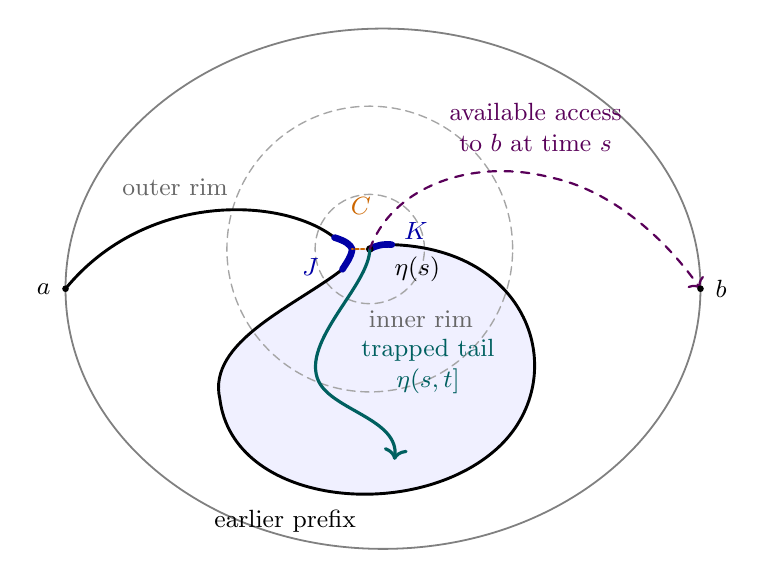
\begin{tikzpicture}[x=1.12cm,y=1.12cm,
    line cap=round,line join=round,font=\small,
    gateprefix/.style={black,line width=1.05pt},
    piece/.style={blue!65!black,line width=2.4pt},
    gate/.style={orange!80!black,line width=1.05pt,densely dotted},
    future/.style={teal!75!black,line width=1.15pt,->},
    access/.style={violet!70!black,line width=.8pt,dashed,->},
    rim/.style={black!35,line width=.5pt,dash pattern=on 3pt off 2pt}]
  \coordinate (a) at (-3.6,0);
  \coordinate (b) at (3.6,0);
  \coordinate (j) at (-.35,.45);
  \coordinate (s) at (-.15,.45);

  \path[fill=blue!6]
    (j) .. controls (-.36,.36) and (-.41,.30) .. (-.46,.22)
    .. controls (-1,-.20) and (-2,-.60) .. (-1.85,-1.25)
    .. controls (-1.70,-2.45) and (.30,-2.65) .. (1.25,-1.85)
    .. controls (2.15,-1.10) and (1.75,.45) .. (.10,.50)
    .. controls (0,.51) and (-.08,.49) .. (s)
    -- (j) -- cycle;

  \draw[black!50,line width=.65pt] (0,0) ellipse (3.6 and 2.95);
  \draw[rim] (s) circle (.62);
  \draw[rim] (s) circle (1.62);
  \node[black!60] at (.43,-.34) {inner rim};
  \node[black!60,anchor=east] at (-1.65,1.15) {outer rim};

  \draw[gateprefix]
    (a) .. controls (-2.70,1.10) and (-1.15,1.05) .. (-.55,.58)
    .. controls (-.42,.54) and (-.37,.50) .. (j)
    .. controls (-.36,.36) and (-.41,.30) .. (-.46,.22)
    .. controls (-1,-.20) and (-2,-.60) .. (-1.85,-1.25)
    .. controls (-1.70,-2.45) and (.30,-2.65) .. (1.25,-1.85)
    .. controls (2.15,-1.10) and (1.75,.45) .. (.10,.50)
    .. controls (0,.51) and (-.08,.49) .. (s);

  \draw[piece]
    (-.55,.58) .. controls (-.42,.54) and (-.37,.50) .. (j)
    .. controls (-.36,.36) and (-.41,.30) .. (-.46,.22);
  \draw[piece]
    (.10,.50) .. controls (0,.51) and (-.08,.49) .. (s);
  \node[blue!65!black,anchor=east] at (-.62,.25) {$J$};
  \node[blue!65!black,anchor=west] at (.13,.65) {$K$};

  \draw[gate] (s) -- (j);
  \node[orange!80!black,anchor=south] at (-.25,.73) {$C$};
  \fill (s) circle (1.35pt);
  \node[anchor=west] at (.02,.22) {$\eta(s)$};

  \draw[future]
    (s) .. controls (-.15,.04) and (-.94,-.60) .. (-.73,-1.05)
    .. controls (-.57,-1.38) and (.19,-1.48) .. (.13,-1.94);
  \node[teal!75!black,align=center] at (.51,-.88)
    {trapped tail\\$\eta(s,t]$};

  \draw[access]
    (s) .. controls (.11,1.17) and (1.03,1.49) .. (1.91,1.26)
    .. controls (2.57,1.12) and (3.18,.60) .. (b);
  \node[violet!70!black,align=center] at (1.73,1.83)
    {available access\\to $b$ at time $s$};

  \fill (a) circle (1.2pt);
  \fill (b) circle (1.2pt);
  \node[anchor=east] at (-3.66,0) {$a$};
  \node[anchor=west] at (3.66,0) {$b$};
  \node[anchor=north] at (-1.11,-2.40) {earlier prefix};
\end{tikzpicture}


 \caption{A small gate with both endpoints on the slit, shown
 schematically.  The endpoints of $C$ lie on an earlier piece $J$
 and a later piece $K$; $\eta(s)$ is the latest endpoint along the
 prefix.  The gate and the intervening prefix enclose the shaded
 region.  A macroscopic tail inside that region crosses the two
 rims, while at time $s$ there is an available route to the target
 on the other side of the gate.  The dashed route denotes this
 possible access, not another sampled continuation.  The annular
 radii and gate width are not drawn to scale.}
 \label{fig:tip-gate}
\end{figure}

Subdivide the curve successively into pieces of diameter less than
$b/100$, by ending a piece when it attains a chosen still smaller
fixed diameter.  Subdivide each of the two original circle arcs
into pieces with the same diameter bound.  The number of curve
pieces is stochastically bounded by
Proposition~\ref{prop:curve-tightness}.  Every gate just constructed
has its two endpoints in a pair $(J,K)$, where $K$ is a later
curve piece and $J$ is an earlier curve piece or a circle piece.
They cannot belong to the same curve piece: that would make the
loop too small to contain the excursion in
\eqref{eq:gate-excursion}.

For each ordered pair use the following revealing stopping rule
during piece $K$: stop the first time in a finite deterministic
schedule that there exists a crosscut of diameter at most $2r$
from the current tip to an earlier point of $J$.  Only non-root
slit endpoints and circle-interior endpoints are admitted.  Such
a schedule can always detect the witness above.  At fixed mesh
there are finitely many complete switch configurations.  For each
configuration exhibiting a witness choose one witness time in an
exploration-compatible clock, and take the union of those finitely
many times.  Although the selections used the full configurations,
their union is a deterministic schedule.  The detection test at
each scheduled time depends only on the current prefix.  It is
therefore a stopping rule, and it occurs no later than the witness
time for the pair in question.  If a time is inside a local piece,
only its already encountered switch is revealed.  A witnessing
crosscut at detection may also be selected deterministically from
the current history.

Let $C_1$ be this first detected crosscut for the witness pair.
We claim that its trapped region and that of $C$ agree outside
$B(\eta_n(s),b/8)$, after taking $r$ sufficiently small.  To prove
this, compare the two closed loops modulo two.  Their long common
prefix segments cancel.  The remaining prefix subarcs lie in $J$
and $K$, and the other remaining arcs are $C$ and $C_1$; in the
circle case there is also a subarc of the one circle piece $J$.
The two pieces have small diameter and are joined by a small
crosscut.  Thus this entire symmetric difference is confined to
the displayed ball.  The winding numbers modulo two of the loops
coincide outside it.  Since each loop is Jordan, its winding
parity is exactly the indicator of its trapped region there.
This proves the claim without any bound on the length or shape of
the intervening common prefix.

The far excursion in \eqref{eq:gate-excursion} consequently visits
the region cut off by $C_1$.  At detection, its tip endpoint has
access to the target side directly across $C_1$ within a ball of
radius $O(r)$.  An excursion reaching the far trapped region
either starts into that region at the detecting tip, or enters
it later through $C_1$, since the other sides of its boundary
belong to the past or the original boundary.  Both entrances
occur inside the inner ball.  The excursion therefore produces a
radial crossing, on the trapped side, from radius $4r$ to a fixed
radius, say $b/3$, about the detection tip.  Outside the inner
ball, the trapped region is bounded only by the past and the
original boundary.  Its annular components therefore cannot
connect to the target-side region without entering the inner
ball.  A route from tip to target is available on the other
side of the gate and avoids all these components, so they are
avoidable.  The argument allows repeated
future crossings of the fictitious crosscut; every such entrance
still occurs inside the inner rim.

By the disk version of Lemma~\ref{lem:macroscopic-avoidability},
the probability of this event for each ordered pair tends to zero
as $r\downarrow0$ after the mesh limit.  To finish, first use
Proposition~\ref{prop:curve-tightness} to bound the number of
pieces with arbitrarily high probability.  The resulting number
of pairs is finite and independent of $r$.  Next choose $r$ to
make the sum of their crossing bounds small, and finally choose
$y$ small enough for the crosscut construction.  This proves
\eqref{eq:tip-approximation} with the asserted order of limits.
\end{proof}

\begin{lemma}[No return from a small target cap]
\label{lem:no-return}
Let $\theta_n(r)$ be the first time $\eta_n$ enters the disk cap
$\D\cap B(1,r)$.  For every $b>0$,
\[
 \lim_{r\downarrow0}\limsup_{n\to\infty}
 \P\bigl(\operatorname{diam}
       \eta_n[\theta_n(r),\infty)>b\bigr)=0.
\]
\end{lemma}

\begin{proof}
At first entrance, the cap has not previously been visited.  It
gives a route from the tip access to the target inside a ball of
radius $O(r)$.  Stop at the entering local piece and allow a
one-step buffer.  A subsequent displacement of diameter $b$
forces a crossing from an enlarged inner rim to a fixed positive
distance, and every relevant annular component is avoidable
because of that tip-to-target route.  Apply
Lemma~\ref{lem:macroscopic-avoidability} in disk coordinates.
This is also the proof of the corresponding target-cap
Corollary in~\cite[Section ``Identification of the Dobrushin
strand'']{C}.  Initial inverse-chart continuity gives the
analogous assertion in physical coordinates.
\end{proof}

\section{Four-mark tests after exploration}\label{sec:slits}

Proposition~\ref{prop:polygon-comparison} concerns a fixed polygon.  The
conditional law seen by an exploration lives instead in a domain whose
boundary contains the entire past of the curve.  We now extend the
four-mark test to these remaining domains.  The main geometric step is
to place the relevant part of such a domain in a compact portion of a
covering surface.  A polygon in that surface still uses the original
square grid, so Proposition~\ref{prop:polygon-comparison} applies to it.

Throughout this Section we fix the deterministic subsequence and the
environment supplied by Lemma~\ref{lem:quenched-diagonal}.  In particular,
the fixed polygon limits hold simultaneously for the countable stock
of rational polygons on finitely many square-grid charts, for both
colors.  All probabilities below are quenched.  Limits of probabilities
are taken along this subsequence; a geometric radius is fixed before
the mesh tends to zero.

We use the simple drawings of Lemma~\ref{lem:compatible-drawing}.  A
\emph{history} is a prefix stopped by a rule that reveals only the
switches encountered by the strand.  Its remaining domain is the
slit disk $U_n$, viewed with its prime-end boundary.  Under separate
primal closure, the two primal boundary intervals are wired separately;
we call them the \emph{electrodes}.  An actual connection between them
uses open edges, together with the identifications within each
electrode.  A \emph{possible connection} means a connection after all
unrevealed edges of the tested color have been allowed, before any
jump along an external wire.  Known bank edges have the physical
accesses described in Lemma~\ref{lem:compatible-drawing}.

\begin{proposition}[Four-mark test in a remaining domain]
\label{prop:moving-test}
Consider the four-change open-cap law and any sequence of
switch-revealing stopping rules before completion of its strand.
Let $A_n$ be events determined by the stopped history.  Suppose that,
on $A_n$, there are basepoints $z_n$ and constants $r_0,\alpha_0>0$,
independent of $n$ and of the history, such that
\begin{enumerate}
\item $B(z_n,r_0)\subset U_n$;
\item in the conformal disk chart normalized at $z_n$, the four
  current prime-end marks, including the tip, have pairwise distance
  at least $\alpha_0$ on the unit circle.
\end{enumerate}
Assume also that the stopped prefixes form a tight family in the
oriented-curve topology, as in Proposition~\ref{prop:curve-tightness}.
Write $\mathcal F_n$ for the stopped information, $E_{\mathrm P}$ for
the primal pairing, and $\chi_{U_n}$ for the ordered cross-ratio of
the four current marks.  Then, for every $t>0$,
\begin{equation}\label{eq:slits-moving-test}
 \P_{\mathrm{open}}\left(
 A_n\cap\left\{
 \left|\P_{\mathrm{open}}(E_{\mathrm P}\mid\mathcal F_n)
             -f(\chi_{U_n})\right|>t\right\}\right)\longrightarrow0.
\end{equation}
The basepoints may be selected from the history.  The original domains
lie in a fixed bounded set, so every deterministic sequence of these
basepoints has a convergent subsequence.
\end{proposition}

The function $f$ is the open-cap function of
Proposition~\ref{prop:pure-four-mark}.  Under separate closure the
corresponding crossing function is
\begin{equation}\label{eq:slits-odds}
 g(\chi)=T(f(\chi)),\qquad
 T(p)=\frac{p}{p+\sqrt2(1-p)}.
\end{equation}
It will suffice to prove an upper bound by $g(\chi_{U_n})$ for the
conditional primal crossing probability.  The identical upper bound
for the dual crossing, together with
$f(1-\chi)=1-f(\chi)$ and the exact conditional change of closure,
will give both sides of \eqref{eq:slits-moving-test}.

\subsection{Physical access and the cost of deleting small balls}

The first two lemmas isolate the probabilistic part of the comparison.
They are the chart and deletion arguments of
\cite[Section ``Alternating tests after exploration'']{C}, with the
one-arm input replaced by Lemma~\ref{lem:full-grid-arm}.  We give their
proofs to specify precisely which boundary identifications are allowed.

Map $U_n$ to
\[
 R_n=(0,1)\times(0,h_n)
\]
so that the electrodes are the vertical sides, and let $u_n$ denote
the first coordinate.  The assumptions of
Proposition~\ref{prop:moving-test} keep $h_n$ in a compact subinterval
of $(0,\infty)$.

\begin{lemma}[Small physical paths have small chart oscillation]
\label{lem:slits-chart}
Under the base-disk and mark-separation assumptions above, there is a
common modulus $\omega(r)\downarrow0$ such that the oscillation of
$u_n$ on any connected path in $U_n$ of physical diameter at most $r$
is at most $\omega(r)$.  The statement includes prime-end accesses by
interior approximation.

Consequently, for every $\beta>0$, a possible connection starting in
\begin{equation}\label{eq:slits-wide-band}
 B_n(\beta)=\{\beta\leq u_n\leq1-\beta\}
\end{equation}
must travel a fixed positive physical distance before reaching an
electrode or a known open bank edge of the tested color, for all
sufficiently small meshes.  The distance is uniform in the history.
\end{lemma}

\begin{proof}
Choose a disk $O$ containing all physical domains with a fixed margin.
For a small ball away from $B(z_n,r_0/2)$, the probability that Brownian
motion from $z_n$ hits that ball before leaving $O$ tends uniformly to
zero with its radius.  For example, the logarithmic harmonic function
in an enclosing annulus gives a bound of order
$1/|\log r|$.  Killing earlier on leaving $U_n$ only decreases this
probability.

In the normalized unit disk, a connected set of diameter at least
$a>0$ has hitting probability from the origin bounded below by a
positive number depending only on $a$.  This is the crosscut form of
the Beurling estimate: a connected set joining two separated small
sectors is either met before exit or separates a boundary interval
of uniformly positive harmonic measure from the origin.  The estimate
also applies to connected sets close to the circle; the set itself,
rather than its boundary projection, lies in the disk.  Conformal
invariance therefore implies that a small physical path away from
the basepoint has small diameter in the disk chart.  Near the basepoint
the same conclusion follows from interior distortion on the fixed
base disk.  The maps from the disk to $R_n$ form a compact family on
the closed disk because the four angles remain separated.  This
proves the asserted modulus for $u_n$.

Every electrode attachment and every known open bank edge has an
access to $u_n=0$ or $u_n=1$ within $O(\delta_n)$, by
Lemma~\ref{lem:compatible-drawing}.  A short possible connection
from $B_n(\beta)$ to such an attachment would, after adding this
access, have chart oscillation at least $\beta$ and physical diameter
tending to zero.  Choose the physical distance so that its modulus
is smaller than $\beta/2$, and then absorb the tile error by taking
$n$ large.  This also shows that the two electrodes have not already
met along the revealed bank under the stated localization.
\end{proof}

\begin{lemma}[Deletion in a central band]\label{lem:slits-deletion}
Fix a history and use separate closure for the tested color.  Delete
a set $S$ of unrevealed edges.  The change in the probability of an
actual electrode-to-electrode connection is at most the original
conditional probability that an endpoint of an edge in $S$ has an
actual connection to an electrode, allowing one edge of $S$ as an
initial test step.

If the deleted incidences lie in $B_n(\beta)$ and in a union of $m$
balls of radius $r$, where $m$ is fixed, this cost tends to zero
uniformly in their centers and in the histories, in the order
\[
 \lim_{r\downarrow0}\limsup_{n\to\infty}.
\]
The same conclusion holds with a fixed number of nested bands and
slightly enlarged balls.
\end{lemma}

\begin{proof}
Couple the original law and the law with the edges in $S$ closed
monotonically.  Explore, in the stronger configuration, the actual
clusters from the deletion endpoints, revealing their incident edges
in both configurations.  FK partition monotonicity remains valid at
each step.  Once these clusters are enclosed by their closed edge
cuts, the conditional laws outside agree and may be coupled
identically.  If no explored cluster reaches an electrode, the
crossing decision is the same.  Known connections along a bank count
as electrode access in this argument.

For the second assertion choose an outer radius $R_\beta>0$ using
Lemma~\ref{lem:slits-chart}.  Every component of possible edges in
a ball of radius $R_\beta$ that meets the deleted central incidences
has no accessible wire or known open attachment there.  All its
remaining boundary identifications arise at the rim of the ball.
Project this graph to the physical grid, fill missing edges, identify
any copies of a physical vertex, and wire the rim.  These operations
increase the induced FK partition and dominate its actual arm event.
Cropping the annulus by a few tile widths accommodates the drawing
and the possible initial test step.  Lemma~\ref{lem:full-grid-arm}
bounds the resulting probability of an arm from radius $r$ to
$R_\beta$ by a quantity tending to zero in the asserted order.  A
union bound over the fixed $m$ balls completes the proof.
\end{proof}

\subsection{Fibers that become crosscuts of a cover}

We next construct a comparison domain without regularizing the slit
boundary itself.  The argument is deterministic.  Consider a sequence
of localized histories whose prefixes converge after increasing
reparametrizations.  The initial boundary curves converge as well.
After passage to a subsequence, the basepoints converge to $z$, the
remaining domains have pointed kernel $U$, their boundaries have a
Hausdorff limit, and the four normalized boundary angles converge.
Here $U$ means the component containing $z$.  The normalized maps
from the disk converge on compact subsets, as do the inverse
rectangle parametrizations, which we denote by
$F_n:R_n\to U_n$.  Every point of $\partial U$ is approached by
complements of $U_n$.  These uses of normalized kernel convergence
and prime-end parametrization are the usual conformal mapping facts; see
\cite{Pommerenke}.

Fix a small trimming parameter $a_*>0$, and then choose
$0<\beta<a_*/20$.  We shall compare the original crossing with a
test between the levels $a_*$ and $1-a_*$.  To control the coordinates
of every possible path between these levels, choose ordered disjoint
abscissa bins, each of width at most $\lambda$ and with every
intervening gap at most $\lambda$, where $\lambda\ll\beta$.
Their convex hull contains
$[2\beta,1-2\beta]$.  Include one bin in $(2\beta,3\beta)$ and one
in $(1-3\beta,1-2\beta)$; the fibers chosen in these two bins will
be called the \emph{anchor fibers}.  These are distinguished members
of the family, not necessarily its extreme fibers; the other bins
may extend beyond them toward the electrodes.

\begin{lemma}[Choice of fibers]\label{lem:slits-fibers}
For every prescribed physical tail radius $r>0$, one can choose a
simple top-to-bottom fiber in each bin, and pass to a subsequence,
with the following properties.
\begin{enumerate}
\item Each fiber stays in its bin in rectangle coordinates.  Apart
  from a top and a bottom tail, it converges inside a compact subset
  of $U$.  Each tail is contained in a physical ball of radius $r$.
\item All physical endpoints of all the fibers have distinct limits.
\item The fibers are mutually disjoint and ordered by their bins.
\end{enumerate}
The omitted top and bottom portions may have fixed, sufficiently
small fractions of the rectangle height.  The two half-fibers may
use different abscissas within the same bin.
\end{lemma}

\begin{proof}
Let $I$ be one bin and let $J$ be a short interval adjacent to the
top or bottom of $R_n$.  By Cauchy--Schwarz,
\begin{equation}\label{eq:slits-length-area}
 \int_I \operatorname{length}
       \bigl(F_n(\{x\}\times J)\bigr)\,dx
 \leq (|I||J|)^{1/2}
       \left(\int_{I\times J}|F_n'(w)|^2\,dA(w)\right)^{1/2}.
\end{equation}
The last integral is at most the area of the common physical
enclosing disk.  By making the height fraction sufficiently small,
the set of levels with tail length exceeding $r$ occupies an
arbitrarily small fraction of $I$.

We can simultaneously separate the endpoints.  On the compact
portions of the horizontal rectangle sides containing the bins,
harmonic measure from the basepoint is uniformly comparable to
abscissa length.  An endpoint in a small physical ball contributes
at most the Brownian probability of reaching that ball before
leaving the enclosing disk.  This tends uniformly to zero as the
ball shrinks, by the logarithmic estimate used in
Lemma~\ref{lem:slits-chart}.  Choose the endpoints successively,
excluding fixed small balls around the endpoints already chosen.
There are only finitely many choices, and these exclusions together
with the length exclusions occupy less than the bin.  A positive
separation can therefore be retained before taking a subsequence.

Choose the top and bottom levels independently, then join them by
an interpolation inside the middle of the same bin.  Interior
convergence of $F_n$ gives convergence of the retained cores after
a further subsequence.  Different bins are disjoint, so the resulting
fibers are disjoint and ordered.  Endpoints can be chosen away from
the finitely many tile corners and exceptional prime accesses.
\end{proof}

Fix an enclosing disk $O$ with a positive margin around all physical
domains.  We enlarge the domain by removing only finitely many
physical points from $O$ and passing to a universal cover.  Include every selected
fiber endpoint among these punctures.  Add finitely many points of
$O\setminus U_n$ whose distinct limits sample $\partial U$ as finely
as required.  Write the resulting set as $P_n$ and its set of
distinct limits as $P$.  Let
\[
 \pi_n:\widetilde O_n\longrightarrow O\setminus P_n
\]
be the universal cover, with a chosen lift of $z_n$.  Its disk
uniformization is normalized by sending $0$ to this lift and making
the derivative of the projection positive at $0$.  Since $U_n$ is
simply connected, its inclusion has a unique lift
\[
 \iota_n:U_n\longrightarrow\widetilde O_n
\]
through the chosen basepoint.  This lift is injective, because
$\pi_n\circ\iota_n$ is the inclusion.  The surface has the ordinary
physical coordinate in every sufficiently small chart; there are
no branch points.

\begin{lemma}[Cover charts and strip trapping]\label{lem:slits-cover}
By choosing the finite boundary sample sufficiently fine, the disk
charts of $\widetilde O_n$ on the retained fiber cores and any fixed
compact access paths in $U$ can be made arbitrarily close to those
of $U_n$, for all sufficiently large $n$.

Give $\widetilde O_n$ rectangle coordinates using the same four disk
angles as for $U_n$, and denote their horizontal coordinate by
$v_n$.  After the tail radius and chart error have been chosen
sufficiently small relative to the bin spacing, each lifted fiber
is a crosscut of the cover rectangle, joining its horizontal sides
and lying in the corresponding abscissa bin with an arbitrarily
small enlargement.  Consequently
\begin{equation}\label{eq:slits-chart-matching}
 |v_n\circ\iota_n-u_n|\leq C\lambda
\end{equation}
between the two extreme fibers.  If $\Gamma_n^-$ and $\Gamma_n^+$
are the first and last fibers, respectively, then
\begin{align*}
 v_n(\iota_n(w))&\leq
     \sup_{\iota_n(\Gamma_n^-)}v_n
       &&\text{on the left electrode side of }\Gamma_n^-,\\
 v_n(\iota_n(w))&\geq
     \inf_{\iota_n(\Gamma_n^+)}v_n
       &&\text{on the right electrode side of }\Gamma_n^+.
\end{align*}
In particular, the enlarged extreme bins bound these coordinates
strictly outside the future test cuts at $a_*$ and $1-a_*$.
\end{lemma}

\begin{proof}
First consider increasingly fine finite samples of $\partial U$.
The normalized projections from the unit disk to the punctured
domains form a bounded normal family.  Their derivative at $0$ is
bounded below by the radius of the common base disk: that disk lifts
to the cover, and Schwarz's lemma gives the derivative comparison.
Any subsequential limit is therefore nonconstant.  Hurwitz's theorem
shows that it omits each point of the dense boundary sample.  Its
image is consequently contained in $U$, the component at $z$.

Conversely, every simply connected domain compactly contained in
$U$ and containing $z$ lifts into all the covers under consideration
once $n$ is large.  The same derivative comparison bounds the
projection derivative below by the conformal radius of that domain.
Exhausting $U$ and then applying Schwarz's lemma to the limit map
into $U$ shows equality with the conformal radius of $U$.  Thus the
limit is precisely the normalized Riemann map onto $U$.  This proves
the asserted approximation on compact sets and along their access
paths.  The order is to fix the desired compact accuracy, choose
a finite puncture list, and only then let $n$ tend to infinity.

For a fixed list with distinct limiting punctures, the charts of
the covers converge under continuation in physical coordinates.
One direct verification is to move the finitely many punctures by
diffeomorphisms supported in disjoint small neighborhoods, fixing
the base disk and the outer boundary, with dilatations tending to
one.  Their lifts, in normalized disk coordinates, converge to the
identity.  On every compact set away from the punctures this
identifies the limiting cover charts and preserves continuation
along any fixed finite collection of paths.

Consider now a fiber tail.  Its projection lies in a ball of radius
$r$ away from the basepoint.  Brownian motion on the cover, projected
to $O$, gives the same upper bound for hitting this tail as for
hitting its physical ball before exit from $O$.  The connected-set
estimate in the unit disk used in Lemma~\ref{lem:slits-chart} thus
makes its diameter small in the cover's disk coordinate.  The
disk-to-rectangle maps form a compact family on the closure, so
its rectangle diameter is small as well.  Apply this observation
to successively shorter tails approaching the endpoint.  The lift
has a continuous endpoint in the closed uniformizing disk.  That
endpoint cannot be interior: its projection tends to a puncture.
It is therefore an ideal boundary point of the cover.

On the retained core, both charts are close to the limiting chart
of $U$.  Taking the omitted height fractions small locates the top
and bottom endpoints near the corresponding horizontal sides,
away from their corners.  The lifted fiber is consequently a
crosscut joining those sides.  Its entire $v_n$-range lies in its
bin with a small enlargement.  These crosscuts are disjoint because
$\iota_n$ is injective, and their order is the order seen on the
common compact cores.

Each crosscut separates the whole cover disk into two components.
The two components of $U_n$ cut by its original fiber lift to the
corresponding sides: each is connected, and the side is determined
on an interior core.  A point between consecutive fibers is
therefore trapped between their lifted crosscuts.  Both its $u_n$
and $v_n$ coordinates lie between the adjacent bins, up to the
chosen errors.  This proves \eqref{eq:slits-chart-matching}.  The
same separation argument outside the two extreme fibers gives the
one-sided bounds.  In particular, the conclusion is global in the
lifted domain; compact convergence alone would not give it.
\end{proof}

\subsection{Keeping the relevant graph in finitely many charts}

The cover has infinitely many sheets.  To apply a fixed polygon test,
we must contain every relevant central incidence in one compact
portion of it.  A bounded physical region and positive puncture
clearance alone would allow arbitrarily many windings around a
puncture.  We will instead construct one access path to each relevant
point with a bounded number of fixed-size displacements; clearance
then bounds the number of chart continuations needed to lift it.
We first delete edges near the finitely many punctures.
The cost of these deletions is controlled by
Lemma~\ref{lem:slits-deletion}; tightness of the histories will control
the number of sheets that remain accessible.

Two different deletions serve this construction.  Removing the
anchor tails forces a central path toward an electrode to cross
a retained anchor core.  The smaller puncture neighborhoods give
the clearance needed to control the lift of that path and its
continuation from the core to the basepoint.  In the whole band
$B_n(\beta)$ make the following deletions:
\begin{enumerate}
\item delete uncertain edges in slightly enlarged balls containing
  the four tails of the two anchor fibers;
\item delete uncertain edges in small balls about every puncture
  of $P_n$.
\end{enumerate}
The tail radius was chosen during Lemma~\ref{lem:slits-fibers}.
Choose the second set of radii only after the finite puncture list
has been fixed.  They may be made small enough that the retained
anchor cores and fixed compact paths joining those cores to the
basepoint have positive clearance from this second set of balls.
No such clearance from the larger tail balls is required of these
auxiliary paths.  All radii are positive and fixed before the mesh
limit.  Lemma~\ref{lem:slits-deletion} makes the total crossing cost
arbitrarily small, first for the four tail balls and then for the
fixed finite number of puncture balls.

In the resulting graph, call an edge or vertex a \emph{candidate}
if its component of possible edges can reach an electrode.  Components
without possible electrode access can be discarded: they cannot
contribute to a crossing or attach to a component that can.

\begin{lemma}[Compact containment of central candidates]
\label{lem:slits-compact-candidates}
After these deletions, all candidate incidences in
$B_n(5\beta)$ lift into a fixed compact part of the limiting cover
charts, for all sufficiently large $n$.
\end{lemma}

\begin{proof}
Start from a central candidate and follow a possible connection
toward an electrode until its first exit from $B_n(\beta)$.
Lemma~\ref{lem:slits-chart} excludes a wire jump before this exit.
The path crosses the anchor fiber on that side.  Up to this crossing
it lies in the band where the puncture-ball edges were deleted, so
it stays away from the punctures.  Its crossing of the anchor cannot
be in a deleted tail.  Following the retained anchor core and then
one of its fixed compact access paths joins the candidate to the
basepoint while still avoiding the smaller puncture balls.  Physical
accesses at vertices can be shifted slightly into $U_n$, retaining
this clearance; tile errors are smaller than every fixed margin.

We show that all points accessible in this way have bounded sheet
indices.  Trim $U_n$ by mutually disjoint disks centered at $P_n$,
with slightly smaller positive radii than the second deletion radii,
and let $T_n$ be the component containing $z_n$.  The preceding paths
put all the central candidates in $T_n$, or in its boundary accesses.
The trimming circles can be chosen in general position, so that
they meet the finite polygonal slit drawing transversely in finitely
many points.

The prime boundary of $T_n$ consists of inherited portions of the
prime boundary of $U_n$, in their original cyclic order, interleaved
with arcs of the trimming circles.  To verify this description, note
that each puncture disk reaches the complement of $U_n$.  A whole
circle surrounding its center cannot lie in the simply connected
domain $U_n$.  Each portion of a trimming circle inside $U_n$ is
therefore a crosscut in the prime-end disk: its two physical
endpoints may coincide on opposite slit banks, but its endpoint
accesses are distinct.  The crosscuts from the disjoint trimming
circles are disjoint, and successive crosscut separation gives the
asserted boundary description of each remaining component.  The
two banks of the slit are counted separately in this description.

The inserted circle arcs have uniformly bounded total length: on
each circle their interiors are disjoint.  The inherited boundary
has a uniform bound on the number of successive oscillations of
every fixed positive size.  Indeed, it consists of the original
boundary traversal and two traversals of the prefix; the original
boundaries converge uniformly and the prefixes belong to a compact
family of curves.  The same oscillation bound holds for the trimmed
boundary.  More explicitly, subdivide the original parametrization
into a bounded number of pieces of diameter less than a prescribed
small fraction of the oscillation scale.  Inherited arcs occur in
that order.  Inserted arcs whose endpoints lie in one such piece
can make a substantial additional excursion only if their length
exceeds a fixed fraction of the scale.  Their number is bounded by
the total circle length.  Arcs crossing subdivision points account
for only a bounded number of further changes.

It remains to turn this boundary control into control of an access
path.  Join a point of $T_n$ and $z_n$ by straight segments to their
first boundary hits, and connect the two resulting prime accesses
along the trimmed boundary.  The straight segments have bounded
length.  The intervening boundary path has the oscillation bound
just established.  Polygonal prime-boundary paths admit arbitrarily
close interior approximations with those accesses, including on
the two sides of a slit.  Thus one obtains an interior path from
$z_n$ to the point with uniformly bounded oscillation count at a
fixed scale smaller than its clearance from every puncture.  An
additional arbitrarily short access segment handles a boundary
incidence.

Cover the common compact physical region away from the punctures
by finitely many ordinary chart disks, smaller than this clearance.
Subdivide the access path whenever its diameter reaches a still
smaller fixed scale.  There are boundedly many pieces, and each
lies in one of these ordinary disks.  Its lift is obtained by a
bounded number of continuations among a finite list of charts,
so it lies in a compact part of the universal cover.  The same
compact chart bound works for the varying punctures by
Lemma~\ref{lem:slits-cover}.  Only one controlled access path is
needed for each point: any other path in $U_n$ reaches the same
lift because $\iota_n$ is single-valued.  This proves the lemma.
\end{proof}

\begin{figure}[t]
\centering
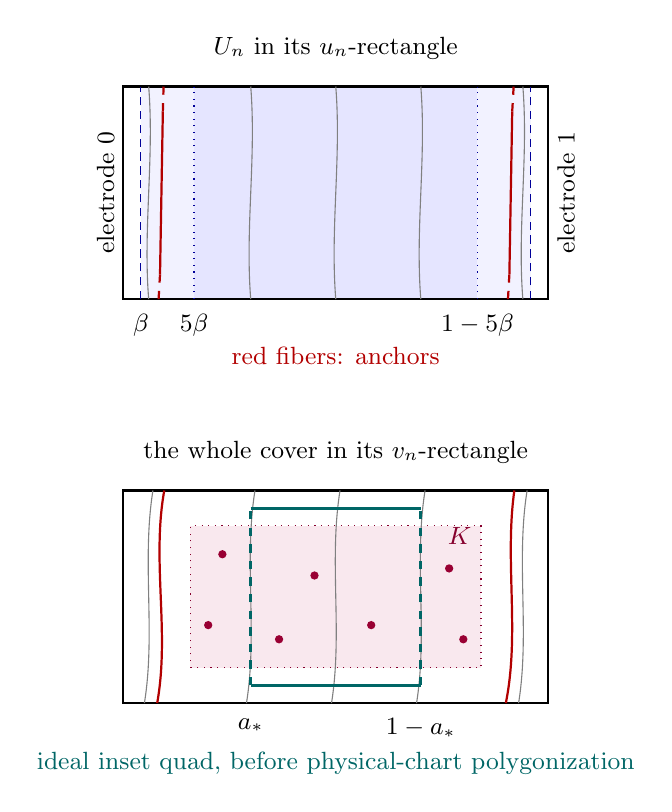
\begin{tikzpicture}[x=0.9cm,y=0.9cm,>=stealth,
  every node/.style={font=\small}]
\begin{scope}
 \fill[blue!5] (0.25,0) rectangle (5.75,3);
 \fill[blue!10] (1,0) rectangle (5,3);
 \draw[thick] (0,0) rectangle (6,3);
 \draw[blue!60!black,densely dashed] (0.25,0)--(0.25,3);
 \draw[blue!60!black,densely dashed] (5.75,0)--(5.75,3);
 \draw[blue!60!black,dotted] (1,0)--(1,3);
 \draw[blue!60!black,dotted] (5,0)--(5,3);
 \foreach \x in {0.36,1.8,3,4.2,5.64} {
  \draw[gray] (\x,0) .. controls (\x-0.08,1) and (\x+0.08,2) .. (\x,3);
 }
 \draw[red!70!black,thick] (0.52,0.35)--(0.56,2.65);
 \draw[red!70!black,thick] (5.45,0.35)--(5.49,2.65);
 \draw[red!70!black,thick,dashed] (0.50,0)--(0.52,0.35);
 \draw[red!70!black,thick,dashed] (0.56,2.65)--(0.57,3);
 \draw[red!70!black,thick,dashed] (5.43,0)--(5.45,0.35);
 \draw[red!70!black,thick,dashed] (5.49,2.65)--(5.51,3);
 \node[above] at (3,3.25) {$U_n$ in its $u_n$-rectangle};
 \node[rotate=90] at (-0.25,1.5) {electrode $0$};
 \node[rotate=90] at (6.25,1.5) {electrode $1$};
 \node[below] at (0.25,-0.08) {$\beta$};
 \node[below] at (1,-0.08) {$5\beta$};
 \node[below] at (5,-0.08) {$1-5\beta$};
 \node[red!70!black] at (3,-0.8) {red fibers: anchors};
\end{scope}
\begin{scope}[shift={(0,-5.7)}]
 \draw[thick] (0,0) rectangle (6,3);
 \fill[purple!9] (0.95,0.5) rectangle (5.05,2.5);
 \draw[purple!70!black,dotted] (0.95,0.5) rectangle (5.05,2.5);
 \draw[red!70!black,thick] (0.48,0)
  .. controls (0.66,1) and (0.40,2) .. (0.58,3);
 \draw[red!70!black,thick] (5.40,0)
  .. controls (5.60,1) and (5.38,2) .. (5.52,3);
 \foreach \x in {0.36,1.8,3,4.2,5.64} {
  \draw[gray] (\x-0.06,0)
   .. controls (\x+0.1,1) and (\x-0.1,2) .. (\x+0.06,3);
 }
 \draw[teal!80!black,very thick] (1.8,0.25)--(4.2,0.25);
 \draw[teal!80!black,very thick] (1.8,2.75)--(4.2,2.75);
 \draw[teal!80!black,very thick,dashed] (1.8,0.25)--(1.8,2.75);
 \draw[teal!80!black,very thick,dashed] (4.2,0.25)--(4.2,2.75);
 \foreach \x/\y in {1.2/1.1,1.4/2.1,2.2/0.9,2.7/1.8,3.5/1.1,4.6/1.9,4.8/0.9} {
  \fill[purple!80!black] (\x,\y) circle (1.5pt);
 }
 \node[above] at (3,3.25) {the whole cover in its $v_n$-rectangle};
 \node[below] at (1.8,-0.08) {$a_*$};
 \node[below] at (4.2,-0.08) {$1-a_*$};
 \node[purple!70!black,anchor=east] at (5.05,2.36) {$K$};
 \node[teal!80!black,align=center] at (3,-0.85)
  {ideal inset quad, before physical-chart polygonization};
\end{scope}
\end{tikzpicture}
\caption{Coordinate trapping and compact containment, schematically
and not to scale;
only a few of the finely spaced fibers are shown.
Fibers in separated bins become ordered crosscuts of the universal
cover; their coordinates agree up to the error in
\eqref{eq:slits-chart-matching}, not exactly.  Their separation
controls the coordinates throughout the lifted domain.  After the deletions, the central candidates lie in a
compact set $K$, shown inside a rectangular compact enclosure in the
lower panel.  The horizontal test sides can therefore be inset by
less than their distance from $K$.  Candidates may extend past both
vertical cuts; those exterior pieces may attach only to the wired
test electrodes.  The teal rectangle is the ideal inset quad; it
is subsequently approximated by a fixed orthogonal polygon in
physical-coordinate charts.  Dashed anchor ends in the upper panel indicate
the tails covered by deletion balls in physical coordinates.}
\label{fig:slits-cover}
\end{figure}

\subsection{A fixed polygon and its FK comparison}

We can now choose the polygon to which the fixed-domain theorem will
be applied.  In the limiting cover rectangle, cut at
$v=a_*$ and $v=1-a_*$.  Place the horizontal sides a small positive
distance inside the top and bottom.  By
Lemma~\ref{lem:slits-compact-candidates}, this distance can be chosen
so small that every central candidate lies strictly on the inner
side of both horizontal walls, with a positive margin.  The resulting
quad is relatively compact in the cover.  Figure~\ref{fig:slits-cover}
shows the distinction between this horizontal containment and the
two vertical cuts, across which candidate paths are allowed to pass.

Approximate the quad by a rational horizontal--vertical polygon
in physical-coordinate charts, with still smaller error and a compact
collar.  Such approximations can be constructed first by polygonal
curves, then by staircases in disjoint thin corridors, and finally
by joining the staircases in disjoint small vertex neighborhoods.
The marked points can be put in straight side interiors.  Uniform
Jordan convergence in a disk chart of the surface implies convergence
of the marked moduli.  Thus the approximation errors can be chosen
after all the preceding margins have been fixed.

\begin{lemma}[The comparison polygon is a fixed test]
\label{lem:slits-fixed-test}
The polygon just constructed may be chosen from the countable stock
in Lemma~\ref{lem:quenched-diagonal}.  For all sufficiently large $n$,
its rounded graph on the varying cover uses the same finite system
of physical-coordinate charts and the same incidence data.  Its
quenched crossing probability therefore converges to the pure
four-mark value for this fixed polygon.
\end{lemma}

\begin{proof}
A compact collared polygon away from the punctures is covered by
finitely many ordinary projection charts.  Choose rational rectangles
inside these charts, with overlaps large enough for the required
continuations.  Their gluings have identity projection transitions.
Subdividing further, the polygon and a collar can be specified by
finitely many rational rectangles or squares, their sheet labels,
and the incidence identifications on overlaps.  There are countably
many finite descriptions of this kind, including when projections
of different sheets overlap.

These finite chart continuations stay a positive distance from the
limiting punctures.  As the punctures move, the same projected paths
and neighborhoods avoid them, and their lift identifications agree
for all large $n$, by the finite-list continuity in
Lemma~\ref{lem:slits-cover}.  Thus both the physical polygon and its
square-grid rounding have fixed chart and incidence descriptions.
Copies of the same physical edge have the same disorder, exactly
as in Proposition~\ref{prop:polygon-comparison}; they are distinct
FK edges when they lie on different sheets.  The simultaneous
fixed-test limit on the chosen environment, followed by
Proposition~\ref{prop:pure-four-mark}, gives the assertion.
\end{proof}

The next comparison is between finite FK graphs, before any limit is
taken.  Let $H_n$ be the conditional graph after the deletions and
discard the components without possible electrode access.  Let
$Q_n$ be the rounded fixed test on the cover.  An edge is
\emph{shared} if it is a remaining central candidate edge of $H_n$
and its lift is an edge of $Q_n$.  We include all edges in the closure
of the rounded test, so an edge path leaving through a vertical
side has a vertex on the corresponding test electrode.

\begin{lemma}[Comparison on shared edges]\label{lem:slits-shared}
For sufficiently small geometric errors and sufficiently large $n$,
\begin{equation}\label{eq:slits-shared-comparison}
 \phi_{H_n}(\text{actual original-electrode crossing})
 \leq
 \phi_{Q_n}^{\mathrm{sep}}(\text{test-electrode crossing}),
\end{equation}
where $\phi_{H_n}$ is the conditional FK law and the two test
electrodes are wired separately in $\phi_{Q_n}^{\mathrm{sep}}$.
\end{lemma}

\begin{proof}
Take the central range for shared edges inside $B_n(5\beta)$,
allowing fixed smaller margins at its boundary.  Since
$\beta<a_*/20$, this range extends well past both vertical test
cuts.  The chart errors in
\eqref{eq:slits-chart-matching} and the polygonization error are
chosen much smaller than these margins.

There is no attachment from a shared edge to a nonshared original
piece through a horizontal test side.  Indeed, every possible
central attachment belongs to the compact candidate set, which
lies on the inner side of those walls with positive clearance.
A noncentral piece cannot enter there either: the global strip
trapping and its one-sided bounds put such pieces beyond the
corresponding vertical cut.  Consequently a nonshared original
piece can attach to the shared graph only along one of the two
test electrodes.

Nor can a nonshared piece connect the two electrodes to each other.
Between small neighborhoods of the vertical cuts there is a middle
strip in which every candidate edge is shared.  A possible path
from the left exterior group to the right must traverse that strip,
by \eqref{eq:slits-chart-matching}.  All identifications from known
banks and original wires belong to the separate left and right
groups: Lemma~\ref{lem:slits-chart} excludes a central access to
either wire and excludes an already known connection between them.

These statements remain valid when the drawing is matched to
physical lattice vertices.  Each uncertain switch supplies only
one random edge, by Lemma~\ref{lem:compatible-drawing}.  For a
primal-open switch, the primal bank follows the revealed ordinary
edge, attaching both endpoint vertex regions to that bank.  For a
primal-closed switch, the encountered turn cuts off only its visited
primal corner, where the bank stays at the same vertex.  The opposite,
unvisited corner retains a connected small neighborhood of its
incidences.  If that other turn is visited later, the same rule then
attaches its corner to the bank.  Thus every vertex whose required
identifications have been separated by the explored strand is
already bank-attached and is excluded from the central band by
Lemma~\ref{lem:slits-chart}.

The boundary construction retains all interior incidences of a
primal boundary vertex.  Exterior dual tabs are separate vertices
of the drawn graph.  Apart from the prescribed electrode-wire
identifications already handled above, distinct tabs require no
identification with one another, and the comparison does not merge
their different lifts.  If two such copies occupy the same ordinary
vertex in one lifted test chart, their merger in the test only
strengthens the local partition.  Interchanging the two colors
gives the same switch argument for a dual test.
Consequently all identifications required among the remaining
unbanked incidences have representatives in a common small vertex
neighborhood.  Away from the puncture balls these representatives
have a common local lift, identical to that of the ordinary grid
incidences.  No additional central identification can therefore join
different sheets or connect the two exterior groups around the shared strip.

Condition now on all nonshared original edges.  Their induced
partition on the shared graph identifies vertices only within
one test electrode or within the other.  It is therefore dominated
by the partition that wires each test electrode separately.
The weights on every shared edge are exactly those in $Q_n$.
Adding the remaining test edges and applying FK monotonicity gives
a stochastic upper comparison on the shared graph.  Finally, every
actual original crossing contains a shared-edge crossing between
the two test electrodes: take its traversal from the left exterior
group to the right, and use the absence of any nonshared bypass.
This event inclusion and the conditional stochastic comparison prove
\eqref{eq:slits-shared-comparison} after averaging the conditioned
edges.  The proof is unchanged for the dual grid and its actual odds.
\end{proof}

\subsection{Completion of the moving test and order of limits}

\begin{proof}[Proof of Proposition~\ref{prop:moving-test}]
Suppose that \eqref{eq:slits-moving-test} fails with a fixed positive
error and a fixed positive probability along a subsequence.
Tightness of the prefixes lets us restrict to a compact family of
curves while losing less than this probability.  In particular,
their numbers of successive displacements of every fixed size
have deterministic bounds on that family.  Select a deterministic
failing history at each remaining mesh.  The initial boundaries
already converge, so we may take the convergent-prefix, basepoint,
angle, and kernel subsequences used above.

It is enough to contradict failure of an upper crossing bound in
one of the two separate closures.  Indeed, if $p_n$ is the
conditional open-cap pairing probability, those crossing
probabilities are exactly $T(p_n)$ and $T(1-p_n)$, respectively,
by Lemma~\ref{lem:cap-change}.  The continuous increasing
map $T$ has a continuous inverse on $[0,1]$.  The two upper bounds
by $g(\chi_{U_n})=T(f(\chi_{U_n}))$ and
$g(1-\chi_{U_n})=T(1-f(\chi_{U_n}))$ therefore force
$p_n-f(\chi_{U_n})\to0$.

Fix an error tolerance.  Choose $a_*$ small, then $\beta<a_*/20$
and the fiber-bin precision $\lambda$ much smaller than $\beta$.
Choose the tail radius so that the four anchor-tail deletions have
small total cost and the lifted tails have sufficiently small chart
diameter.  Lemma~\ref{lem:slits-fibers} gives a fixed finite number
of fibers and their limiting endpoints.  Choose a fixed finite
puncture sample fine enough for Lemma~\ref{lem:slits-cover}.  Only
after that choice, take the puncture-ball radii small enough for
both the required core clearances and a small total deletion cost.
Lemma~\ref{lem:slits-compact-candidates} then gives one compact
part of the cover containing the surviving central candidates.
Choose the horizontal inset of the test smaller than the clearance
of this compact set, and finally choose the rational polygon with
strictly smaller approximation errors.

All these data are fixed before taking the mesh limit.  The
deletion bound and Lemmas~\ref{lem:slits-fixed-test}
and~\ref{lem:slits-shared} give
\[
 \limsup_{n\to\infty}
 \left[
 \phi_n^{\mathrm{sep}}(\text{original crossing}\mid\mathcal F_n)
       -g(\chi_{U_n})
 \right]
 \leq \text{deletion error}+\text{modulus error}.
\]
The modulus error tends to zero as the vertical trim $a_*$, the
horizontal inset, and the polygonization error tend to zero.
The cover rectangle was given the same four-angle data as $U_n$,
and all rectangle heights remain in a compact nondegenerate range,
so continuity of the pure four-mark function justifies this
comparison uniformly in the limiting height.  The deletions have
the independently small costs proved above.  The right side can
therefore be made arbitrarily small.  Applying the same argument
to the dual proves the two upper bounds and contradicts the
selected failure.

Although the geometry was selected after fixing an environment and
a failing history subsequence, the polygon used at the last step
is one fixed member of the previously simultaneous countable stock.
No estimate is applied to a boundary that continues to change with
the mesh, and no uniform rate over all polygons is needed.  This
completes the proof for arbitrary stopping rules satisfying the
stated localization and tightness assumptions.
\end{proof}

\section{Identification of the driving process and the ordered curve}
\label{sec:identification}

We remain on the deterministic subsequence and fixed environment of
Lemma~\ref{lem:quenched-diagonal}.  Proposition~\ref{prop:moving-test}
now supplies the four-change crossing probability after localized
exploration.  To extract the Dobrushin driving process from this
probability, we insert a short wired interval on the free boundary.
The pairing martingale belongs to the resulting four-change law.
We first replace it by a bounded Loewner expression, and only then
compare that law with the original Dobrushin law.  This order is
what permits the interval to shrink without amplifying the
comparison error.  The method follows the \emph{Bounded martingale
tests} Lemma and \emph{Driving convergence} Proposition
of~\cite[Section ``Identification of the Dobrushin strand'']{C}.

\subsection{Bounded tests from a shrinking boundary interval}

Use the initial half-plane coordinate
$\psi_n=\Psi\circ\varphi_n$ from Section~\ref{sec:tightness},
reflecting the half-plane picture if necessary so that its positive
real side is primal-free.
Write $g_{n,t}$ and $W_n(t)$ for the maps and driver in
\eqref{eq:loewner-clock}.  Fix $T,R<\infty$ and stop at
$\tau_n=\tau_n(T,R)$.  Write $\E_n$ for expectation under the
original Dobrushin law in the fixed environment.  Let
$\mathcal F_{n,t}$ be the filtration of
the explored path and the switches it has encountered.  For
$x>2R+1$, define
\begin{equation}\label{eq:power-test}
 M_{n,t}(x)=
 \left(\frac{xg'_{n,t}(x)}{g_{n,t}(x)-W_n(t)}\right)^{1/2},
 \qquad 0\le t\le\tau_n.
\end{equation}
The real point $x$ is not swallowed on this range.  Indeed,
$g_{n,t}(x)\ge x$ and
\begin{equation}\label{eq:real-flow-bounds}
 \begin{split}
 x-R&\le g_{n,t}(x)-W_n(t)
       \le x+R+\frac{2T}{x-R},\\
 g'_{n,t}(x)&=
 \exp\left(-\int_0^t
       \frac{2\,du}{(g_{n,u}(x)-W_n(u))^2}\right).
 \end{split}
\end{equation}
Consequently $M_{n,t}(x)$ and its reciprocal are bounded by
constants depending only on $T,R,x$.

\begin{lemma}[Approximate martingale identities]
\label{lem:bounded-martingale-tests}
For each $x>2R+1$, every sequence of revealing stopping times
$0\le\sigma_n\le\upsilon_n\le\tau_n$, and every uniformly bounded
$\mathcal F_{n,\sigma_n}$-measurable sequence $F_n$, the original
Dobrushin law satisfies
\begin{equation}\label{eq:approximate-martingale}
 \E_n\left[
 F_n\bigl(M_{n,\upsilon_n}(x)-M_{n,\sigma_n}(x)\bigr)
 \right]\longrightarrow0.
\end{equation}
Stops during a known local arc are allowed.
\end{lemma}

\begin{proof}
Fix $s>0$, initially without taking a limit in $s$.  Insert a
separate primal wired interval on the formerly free side, with
lattice endpoints whose initial half-plane coordinates tend to
$x,x+s$.  In the open-cap four-change law, explore the strand
starting at the original initial mark $a_n$, whose half-plane
coordinate is $0$.  By
Lemma~\ref{lem:compatible-drawing}, the domain, initial charts,
and drawings may be chosen the same away from this insertion.
Regard the Dobrushin stopping rules and $F_n$ as functions of
revealed histories.  Apply the same rules on the common tree of
prefix histories, extend them as stopping rules outside that tree
by stopping at its first exit, and extend $F_n$ boundedly there.
These conventions retain the order of the two stops and their
localization; below we show that the relevant stopped prefixes
stay in the common tree.  Thus the same symbols will denote
well-defined stopping times and history tests under open caps.

We check the localization required by
Proposition~\ref{prop:moving-test}.  Real Loewner trajectories from
$x$ and $x+s$ remain separated from the driver, and their gap solves
\begin{equation}\label{eq:real-gap}
 \partial_t\bigl(g_{n,t}(x+s)-g_{n,t}(x)\bigr)
 =-\frac{2\bigl(g_{n,t}(x+s)-g_{n,t}(x)\bigr)}
 {(g_{n,t}(x+s)-W_n(t))(g_{n,t}(x)-W_n(t))}.
\end{equation}
For fixed $s$, this gap is bounded below by a positive constant.
The same ODE is regular in a complex neighborhood of the interval,
uniformly on the stopped range.  The prefix therefore stays out
of a fixed neighborhood of the insertion, and cannot terminate
at either inserted mark before the stop.  A point initially
corresponding to $iY$, with $Y$ sufficiently large, has a fixed
disk untouched by all these hulls.  It supplies the basepoint of
Proposition~\ref{prop:moving-test}.  The four marks, including tip
and infinity, are uniformly separated in the normalized charts
for each fixed $s$.  Initial marked Jordan convergence transfers
these statements to the physical drawings.  The history
tightness hypothesis follows from
Proposition~\ref{prop:curve-tightness} for the four fixed marks.

Let $Z_{n,t}^{s}$ be the conditional probability of the rare primal
pairing under the open-cap law.  It is an exact bounded
martingale in the revealed-switch filtration.  At each of the
allowed stopping times,
Proposition~\ref{prop:moving-test} gives
\begin{equation}\label{eq:four-mark-replacement}
 Z_{n,t}^{s}-f(\chi_{n,t}^{s})\longrightarrow0
 \quad\hbox{in probability and in mean},\qquad
 \chi_{n,t}^{s}=
 \frac{g_{n,t}(x+s)-g_{n,t}(x)}
      {g_{n,t}(x+s)-W_n(t)}.
\end{equation}
The vanishing initial errors in the lattice mark positions are
included here; they do not affect the fixed-$s$ limit.
Optional sampling and the boundedness of $F_n$ thus give the
approximate martingale identity for $f(\chi_{n,t}^{s})$.

Divide this identity by $f(s/(x+s))$ while $s$ is fixed.  The
small-interval behavior in
Proposition~\ref{prop:pure-four-mark}, together with analytic ODE
bounds near $x$, gives
\begin{equation}\label{eq:normalized-small-interval}
 \frac{f(\chi_{n,t}^{s})}{f(s/(x+s))}
       =M_{n,t}(x)+o_s(1)+o_n(1).
\end{equation}
Here $o_n(1)$ is taken first for fixed $s$, and $o_s(1)$ is uniform
over the stopped paths.  More explicitly,
\[
 \frac{\chi_{n,t}^{s}}{s/(x+s)}
 =\frac{xg'_{n,t}(x)}{g_{n,t}(x)-W_n(t)}+O(s),
\]
with the ratio bounded above and away from zero; applying
$f(u)\sim c\sqrt u$ proves the displayed replacement.  By
\eqref{eq:real-flow-bounds}, the expression after replacement is
bounded independently of small $s$.

We can now compare laws using only bounded functions of the
stopped histories.  First compare the deterministic separate
primal closure with the Dobrushin law.  The former adds just the
short wired interval, so FK monotonicity gives a coupling.
Explore its actual open clusters in the stronger law.  Unless
one reaches a fixed outer neighborhood of the insertion, the
configurations outside that neighborhood can be coupled
identically: the explored clusters are enclosed by closed cuts,
and the conditional outside laws then agree.  The insertion has
physical diameter tending to zero as $s\downarrow0$, by the
uniform continuity of the initial inverse maps.  The old primal
wire stays a positive distance away.  The intervening annulus
therefore has no primal wire attachments except at its rims,
and Lemma~\ref{lem:full-grid-arm} shows that the probability of
reaching the outer neighborhood tends to zero, first in the mesh
limit and then as $s\downarrow0$.

Second, compare this deterministic closure to open caps.
Lemma~\ref{lem:cap-change} gives a likelihood depending only on
the pairing, with two fixed positive values.  If the exceptional
pairing has probability $p$ under the separate-closure law,
normalizing these two weights
shows that the total variation difference is at most $C p$.
By Proposition~\ref{prop:moving-test} at the empty prefix and
Lemma~\ref{lem:cap-change}, for fixed $s$ that separate-closure
pairing probability tends to
$g(s/(x+s))$, which tends to zero as $s\downarrow0$.

The stopped prefixes avoid the spare neighborhood of the
insertion established above.  On the successful coupling event
their drawings, revealed histories, Loewner maps, and stopping
rules therefore agree.  The extension convention also makes
the stopped tests agree on these common histories.  Combining the two comparisons with
\eqref{eq:normalized-small-interval} yields
\[
 \limsup_{n\to\infty}
 \left|\E_n\!\left[
 F_n(M_{n,\upsilon_n}(x)-M_{n,\sigma_n}(x))\right]\right|
 \le e(s),\qquad \lim_{s\downarrow0}e(s)=0.
\]
This proves \eqref{eq:approximate-martingale}.  Notice that the
coupling errors were applied after replacement by bounded tests;
they were never divided by the small number $f(s/(x+s))$.
\end{proof}

\subsection{Two tests determine the driver}

\begin{proposition}[Driving convergence]
\label{prop:driving-convergence}
In the fixed environment under consideration, $W_n$ converges in
law, uniformly on compact capacity intervals, to
$\sqrt{16/3}\,B$, where $B$ is standard real Brownian motion.
\end{proposition}

\begin{proof}
We first prove tightness under the fixed localization $T,R$.
Set $h=1/2$ and, for $x>2R+1$, write
\[
 X_{n,t}(x)=g_{n,t}(x),\qquad
 A_{n,t}(x)=x^h g'_{n,t}(x)^h,\qquad
 M_{n,t}(x)=A_{n,t}(x)(X_{n,t}(x)-W_n(t))^{-h}.
\]
The real-flow bounds show that $X_n,A_n$ are uniformly bounded
and Lipschitz in time, with $A_n$ bounded away from zero.
Choose $2R+1<x_1<x_2$.  Equation~\eqref{eq:real-gap} also gives
a positive lower bound on
$X_{n,t}(x_2)-X_{n,t}(x_1)$ throughout the stopped range.

At a revealing stopping time $\sigma_n$, freeze these two
quantities and define, for $-R\le w\le R$,
\[
 F_j(w)=A_{n,\sigma_n}(x_j)
       (X_{n,\sigma_n}(x_j)-w)^{-h},\qquad j=1,2.
\]
Both derivatives are positive.  Their ratio is
\[
 r(w):=\frac{F'_1(w)}{F'_2(w)}
 =\frac{A_{n,\sigma_n}(x_1)}{A_{n,\sigma_n}(x_2)}
 \left(\frac{X_{n,\sigma_n}(x_2)-w}
            {X_{n,\sigma_n}(x_1)-w}\right)^{h+1}.
\]
The separation of the two real solutions and their uniform
bounds imply $r'(w)\ge c>0$.  Also $F'_2(w)$ is bounded above
and away from zero.  Put
$a_n=r(W_n(\sigma_n))$.  Integrating
$F'_2(w)(r(w)-a_n)$ on either side of $W_n(\sigma_n)$ gives
\begin{equation}\label{eq:two-test-convexity}
 F_1(w)-F_1(W_n(\sigma_n))
 -a_n\bigl(F_2(w)-F_2(W_n(\sigma_n))\bigr)
 \ge c_1|w-W_n(\sigma_n)|^2.
\end{equation}
The predictable coefficient $a_n$ is uniformly bounded.

Between $\sigma_n$ and another allowed stop $\upsilon_n$, changing
the frozen $X_n,A_n$ costs at most
$C(\upsilon_n-\sigma_n)$.  Apply
Lemma~\ref{lem:bounded-martingale-tests} to the two increments,
using the bounded $\mathcal F_{n,\sigma_n}$-measurable coefficient
$a_n$ as a test for the second.  Equation~\eqref{eq:two-test-convexity}
then yields
\begin{equation}\label{eq:driver-increment}
 \E_n|W_n(\upsilon_n)-W_n(\sigma_n)|^2
 \le C\E_n(\upsilon_n-\sigma_n)+o(1).
\end{equation}
This holds for every sequence of allowed stopping times.  In
particular, for the driver stopped at $\tau_n$, it implies the
stopping-time tightness criterion of Aldous~\cite{Aldous} in the
Skorokhod $J_1$ topology.
The drivers are bounded on this range.  Every prelimit driver is
continuous, and the continuous paths form a closed subspace for
$J_1$ convergence.  Thus all limits are continuous, and convergence
along a subsequence may be realized uniformly on compact stopped
intervals.

We identify any such limit inside an inner driver bound, choosing
inner levels which are continuity levels for the stopping operation.
These levels can be increased to the outer bound.  Continuity of
the Loewner ODE under uniform driver convergence gives limits
$X_t(x),A_t(x)$ and
\begin{equation}\label{eq:limiting-power-test}
 M_t(x)=A_t(x)(X_t(x)-W_t)^{-h}.
\end{equation}
Use bounded continuous functions of finitely many earlier driver
values as tests in \eqref{eq:approximate-martingale}, and then a
monotone-class argument.  It follows that each $M(x)$ is a
martingale in the limiting filtration.  This argument applies at
the localized stops as well.  The bounds above and below persist.

Before applying It\^o's formula, note that
\[
 W_t=X_t(x)-\left(\frac{A_t(x)}{M_t(x)}\right)^{1/h}.
\]
The processes $X,A$ are continuous of finite variation, $M$ is a
continuous martingale, and the function in this identity is smooth
on the range of their positive bounds.  Hence $W$ is a continuous
semimartingale.  Write its decomposition as a continuous local
martingale plus a continuous finite-variation process $B^{\rm fv}$,
and denote its quadratic variation by $[W]$.

Put $Z_t(x)=X_t(x)-W_t$.  The Loewner equations give
\[
 dX_t(x)=2Z_t(x)^{-1}\,dt,\qquad
 d\log A_t(x)=-2hZ_t(x)^{-2}\,dt.
\]
The finite-variation part of $dM_t(x)/M_t(x)$ is consequently
\[
 hZ_t(x)^{-1}\,dB_t^{\rm fv}
 -4hZ_t(x)^{-2}\,dt
 +\frac{h(h+1)}{2}Z_t(x)^{-2}\,d[W]_t.
\]
It vanishes because $M(x)$ is a martingale.  Multiplication by
$Z_t(x)^2/h$ gives an identity of signed measures,
\begin{equation}\label{eq:driver-characteristics}
 Z_t(x)\,dB_t^{\rm fv}-4\,dt
      +\frac{1+h}{2}\,d[W]_t=0.
\end{equation}
Subtract this identity for $x_1$ and $x_2$.  Their strictly
positive separation forces $dB^{\rm fv}=0$.  Substitution back
into \eqref{eq:driver-characteristics} yields
\[
 d[W]_t=\frac{8}{1+h}\,dt=\frac{16}{3}\,dt.
\]
L\'evy's characterization therefore identifies the stopped limit
as Brownian motion with variance rate $16/3$.  If the initial
half-plane picture was reflected, reflecting back negates the
driver and leaves this Brownian law unchanged.

It remains to remove the outer driver bound.  For any fixed
capacity horizon, the limiting upper bound on the probability
that $W_n$ exits $[-R,R]$ is bounded by the Brownian probability
of reaching inner levels tending to $R$.  This follows by applying
the stopped convergence at continuity levels below $R$; exiting
the outer interval entails first reaching each such inner level.
These Brownian probabilities tend to zero as $R\to\infty$.
Thus the full drivers are tight on every compact capacity
interval, and each subsequential law has the Brownian
identification just proved.  This proves the proposition.
\end{proof}

\subsection{From capacity time to the full oriented curve}

We can now complete the proof of Theorem~\ref{thm:main}.  We first
work in the common disk, and then return to the physical domains
and to environmental probability.

\begin{proof}[Proof of Theorem~\ref{thm:main}]
Fix the environment and subsequence of
Lemma~\ref{lem:quenched-diagonal}.  By
Proposition~\ref{prop:driving-convergence}, the drivers converge
uniformly on compact time intervals in law to
$W=\sqrt{16/3}\,B$.  For every fixed height $y>0$, continuity of
the inverse Loewner equation gives convergence of
\[
 H_n(t,y)=\Psi^{-1}\!\left(g_{n,t}^{-1}(W_n(t)+iy)\right)
\]
uniformly in $t$ on each compact capacity interval to the analogous
$H(t,y)$ for $W$.  A large driver bound has arbitrarily high
probability on that interval, so
Proposition~\ref{prop:tip-approximation} applies after localization.

For completeness, the uniform conclusion at height zero follows
without assuming uniform boundary convergence of the inverse
maps.  For two small positive heights, the triangle inequality
and \eqref{eq:tip-approximation} show that $H_n(\cdot,y)$ and
$H_n(\cdot,y')$ are close in the uniform metric, in probability,
after the mesh limit.  Passing at these fixed heights to the
limiting driver proves that $H(\cdot,y)$ is Cauchy in probability
in the space of continuous disk-valued functions on the time
interval as $y\downarrow0$.  Its limit is continuous.  The SLE
trace theorem~\cite{RS} identifies its pointwise values with the
SLE trace, first at rational times and then at all times by
continuity.  The same approximation argument now gives
\begin{equation}\label{eq:capacity-trace-convergence}
 \eta_n\ \Longrightarrow\ \eta
 \quad\hbox{uniformly on every compact capacity interval},
\end{equation}
where $\eta$ is chordal $\mathrm{SLE}_{16/3}$ in $\D$ from $-1$
to $1$.  In particular, a macroscopic excursion cannot be hidden
in a sequence of capacity intervals of vanishing length: the
uniform tip estimate already controls all times in those intervals.

To include the terminal part of the curve, first fix a small cap
about $1$.  Chordal SLE tends to its target almost surely
\cite{RS}; hence with probability as close to one as desired its
tail after a sufficiently large deterministic time lies in a
smaller cap.  By \eqref{eq:capacity-trace-convergence}, the
discrete curve has entered the original cap by that time with
the same high probability.  Lemma~\ref{lem:no-return} bounds
the diameter of its subsequent tail.  Letting the cap shrink
therefore makes both tails uniformly small.  Parametrize the
two curves by the common capacity clock until the chosen time
and then by any increasing parametrizations of their tails.
This proves convergence in the full uniform oriented-curve
metric modulo increasing reparametrization.

The initial inverse disk charts converge uniformly on their
closures by marked Jordan convergence.  Composing with them
transfers the curve convergence to the original physical
embedding.  Finally, the drawing comparison gives
$d(\gamma_n,\widehat\gamma_n)=O(\delta_n)$ in that same oriented
metric.  We have proved the asserted weak convergence of
quenched laws for every environment in the full-probability
event of Lemma~\ref{lem:quenched-diagonal}.

Return now to the entire prescribed mesh sequence.  The
oriented-curve space, with constant waiting intervals identified,
is separable, and its weak probability-law topology is metrized
by the bounded-Lipschitz distance for the bounded curve metric.
Each finite quenched law is measurable in its bonds.  From every
subsequence, Lemma~\ref{lem:quenched-diagonal} selects a further
deterministic subsequence along which this distance from the SLE
law tends to zero almost surely.  The subsequence criterion for
convergence in probability proves convergence in environmental
probability along the full sequence.  All choices requiring
small disorder were made before choosing the domain and its
approximation, as in the polygon comparison.  This completes
the proof.
\end{proof}

\begin{thebibliography}{99}

\bibitem{Aldous}
D.~Aldous,
\emph{Stopping times and tightness},
Ann. Probab. \textbf{6} (1978), 335--340.

\bibitem{AM}
E.~Av\'erous and R.~Mahfouf,
\emph{The near-critical random bond FK-percolation model},
preprint (2025), \href{https://arxiv.org/abs/2509.08938}{arXiv:2509.08938}.

\bibitem{CDH}
D.~Chelkak, H.~Duminil-Copin, and C.~Hongler,
\emph{Crossing probabilities in topological rectangles for the critical planar FK-Ising model},
Electron. J. Probab. \textbf{21} (2016), paper no.~5, 28~pp.
\href{https://doi.org/10.1214/16-EJP3452}{doi:10.1214/16-EJP3452}.

\bibitem{CDHKS}
D.~Chelkak, H.~Duminil-Copin, C.~Hongler, A.~Kemppainen, and S.~Smirnov,
\emph{Convergence of Ising interfaces to Schramm's SLE curves},
C. R. Math. Acad. Sci. Paris \textbf{352} (2014), 157--161.
\href{https://doi.org/10.1016/j.crma.2013.12.002}{doi:10.1016/j.crma.2013.12.002}.

\bibitem{CI}
D.~Chelkak and K.~Izyurov,
\emph{Holomorphic spinor observables in the critical Ising model},
Comm. Math. Phys. \textbf{322} (2013), 303--332.
\href{https://doi.org/10.1007/s00220-013-1763-5}{doi:10.1007/s00220-013-1763-5}.

\bibitem{CS}
D.~Chelkak and S.~Smirnov,
\emph{Universality in the 2D Ising model and conformal invariance of fermionic observables},
Invent. Math. \textbf{189} (2012), 515--580.
\href{https://doi.org/10.1007/s00222-011-0371-2}{doi:10.1007/s00222-011-0371-2}.
Theorem and equation locators agree with
\href{https://arxiv.org/abs/0910.2045v2}{arXiv:0910.2045v2}.

\bibitem{DD}
Vik.~S.~Dotsenko and Vl.~S.~Dotsenko,
\emph{Critical behaviour of the 2D Ising model with impurity bonds},
J. Phys. C: Solid State Phys. \textbf{15} (1982), 495--507.
\href{https://doi.org/10.1088/0022-3719/15/3/015}{doi:10.1088/0022-3719/15/3/015}.

\bibitem{DCHN}
H.~Duminil-Copin, C.~Hongler, and P.~Nolin,
\emph{Connection probabilities and RSW-type bounds for the two-dimensional FK Ising model},
Comm. Pure Appl. Math. \textbf{64} (2011), 1165--1198.
\href{https://doi.org/10.1002/cpa.20370}{doi:10.1002/cpa.20370}.

\bibitem{ES}
R.~G.~Edwards and A.~D.~Sokal,
\emph{Generalization of the Fortuin--Kasteleyn--Swendsen--Wang representation and Monte Carlo algorithm},
Phys. Rev. D \textbf{38} (1988), 2009--2012.
\href{https://doi.org/10.1103/PhysRevD.38.2009}{doi:10.1103/PhysRevD.38.2009}.

\bibitem{FK}
C.~M.~Fortuin and P.~W.~Kasteleyn,
\emph{On the random-cluster model. I. Introduction and relation to other models},
Physica \textbf{57} (1972), 536--564.
\href{https://doi.org/10.1016/0031-8914(72)90045-6}{doi:10.1016/0031-8914(72)90045-6}.

\bibitem{FKG}
C.~M.~Fortuin, P.~W.~Kasteleyn, and J.~Ginibre,
\emph{Correlation inequalities on some partially ordered sets},
Comm. Math. Phys. \textbf{22} (1971), 89--103.
\href{https://doi.org/10.1007/BF01651330}{doi:10.1007/BF01651330}.

\bibitem{Harris}
A.~B.~Harris,
\emph{Effect of random defects on the critical behaviour of Ising models},
J. Phys. C: Solid State Phys. \textbf{7} (1974), 1671--1692.
\href{https://doi.org/10.1088/0022-3719/7/9/009}{doi:10.1088/0022-3719/7/9/009}.

\bibitem{Izyurov}
K.~Izyurov,
\emph{Critical Ising interfaces in multiply-connected domains},
Probab. Theory Related Fields \textbf{167} (2017), 379--415.
\href{https://doi.org/10.1007/s00440-015-0685-x}{doi:10.1007/s00440-015-0685-x}.
Theorem and equation locators refer to
\href{https://arxiv.org/abs/1309.5302}{arXiv:1309.5302}.

\bibitem{KS}
A.~Kemppainen and S.~Smirnov,
\emph{Random curves, scaling limits and Loewner evolutions},
Ann. Probab. \textbf{45} (2017), 698--779.
\href{https://doi.org/10.1214/15-AOP1074}{doi:10.1214/15-AOP1074}.

\bibitem{Ludwig}
A.~W.~W.~Ludwig,
\emph{Critical behavior of the two-dimensional random $q$-state Potts model by expansion in $(q-2)$},
Nuclear Phys. B \textbf{285} (1987), 97--142.
\href{https://doi.org/10.1016/0550-3213(87)90330-0}{doi:10.1016/0550-3213(87)90330-0}.

\bibitem{LudwigCorrelations}
A.~W.~W.~Ludwig,
\emph{Infinite hierarchies of exponents in a diluted ferromagnet and their interpretation},
Nuclear Phys. B \textbf{330} (1990), 639--680.
\href{https://doi.org/10.1016/0550-3213(90)90126-X}{doi:10.1016/0550-3213(90)90126-X}.

\bibitem{C}
OpenAI,
\emph{Conformal Limits of Critical Square-Lattice Random-Cluster Interfaces},
OpenAI Math Release preprint
\href{https://github.com/openai/math/blob/main/preprints/Conformal-Limits-of-Critical-Square-Lattice-Random-Cluster-Interfaces-October-5-2026/paper.pdf}{OAI:Conformal-Limits-of-Critical-Square-Lattice-Random-Cluster-Interfaces-October-5-2026},
2026.

\bibitem{Q}
OpenAI,
\emph{Quenched $\mathrm{SLE}_3$ Universality for the Weak Random-Bond Ising Model},
OpenAI Math Release preprint
\href{https://github.com/openai/math/blob/main/preprints/Quenched-SLE3-Universality-for-the-Weak-Random-Bond-Ising-Model-October-5-2026/quenched-sle3-weak-random-bond-ising.pdf}{OAI:Quenched-SLE3-Universality-for-the-Weak-Random-Bond-Ising-Model-October-5-2026},
2026.

\bibitem{Pommerenke}
Ch.~Pommerenke,
\emph{Boundary Behaviour of Conformal Maps},
Grundlehren der mathematischen Wissenschaften, vol.~299,
Springer-Verlag, Berlin, 1992.
\href{https://doi.org/10.1007/978-3-662-02770-7}{doi:10.1007/978-3-662-02770-7}.

\bibitem{RS}
S.~Rohde and O.~Schramm,
\emph{Basic properties of SLE},
Ann. of Math. (2) \textbf{161} (2005), 883--924.
\href{https://doi.org/10.4007/annals.2005.161.883}{doi:10.4007/annals.2005.161.883}.

\bibitem{Shalaev}
B.~N.~Shalaev,
\emph{Critical behavior of the two-dimensional Ising model with random bonds},
Phys. Rep. \textbf{237} (1994), 129--188.
\href{https://doi.org/10.1016/0370-1573(94)90086-8}{doi:10.1016/0370-1573(94)90086-8}.

\bibitem{Smirnov}
S.~Smirnov,
\emph{Conformal invariance in random cluster models. I. Holomorphic fermions in the Ising model},
Ann. of Math. (2) \textbf{172} (2010), 1435--1467.
\href{https://doi.org/10.4007/annals.2010.172.1435}{doi:10.4007/annals.2010.172.1435}.

\end{thebibliography}

\end{document}
